\documentclass[twoside]{book}

% Packages required by doxygen
\usepackage{fixltx2e}
\usepackage{calc}
\usepackage{doxygen}
\usepackage[export]{adjustbox} % also loads graphicx
\usepackage{graphicx}
\usepackage[utf8]{inputenc}
\usepackage{makeidx}
\usepackage{multicol}
\usepackage{multirow}
\PassOptionsToPackage{warn}{textcomp}
\usepackage{textcomp}
\usepackage[nointegrals]{wasysym}
\usepackage[table]{xcolor}

% Font selection
\usepackage[T1]{fontenc}
\usepackage[scaled=.90]{helvet}
\usepackage{courier}
\usepackage{amssymb}
\usepackage{sectsty}
\renewcommand{\familydefault}{\sfdefault}
\allsectionsfont{%
  \fontseries{bc}\selectfont%
  \color{darkgray}%
}
\renewcommand{\DoxyLabelFont}{%
  \fontseries{bc}\selectfont%
  \color{darkgray}%
}
\newcommand{\+}{\discretionary{\mbox{\scriptsize$\hookleftarrow$}}{}{}}

% Page & text layout
\usepackage{geometry}
\geometry{%
  a4paper,%
  top=2.5cm,%
  bottom=2.5cm,%
  left=2.5cm,%
  right=2.5cm%
}
\tolerance=750
\hfuzz=15pt
\hbadness=750
\setlength{\emergencystretch}{15pt}
\setlength{\parindent}{0cm}
\setlength{\parskip}{3ex plus 2ex minus 2ex}
\makeatletter
\renewcommand{\paragraph}{%
  \@startsection{paragraph}{4}{0ex}{-1.0ex}{1.0ex}{%
    \normalfont\normalsize\bfseries\SS@parafont%
  }%
}
\renewcommand{\subparagraph}{%
  \@startsection{subparagraph}{5}{0ex}{-1.0ex}{1.0ex}{%
    \normalfont\normalsize\bfseries\SS@subparafont%
  }%
}
\makeatother

% Headers & footers
\usepackage{fancyhdr}
\pagestyle{fancyplain}
\fancyhead[LE]{\fancyplain{}{\bfseries\thepage}}
\fancyhead[CE]{\fancyplain{}{}}
\fancyhead[RE]{\fancyplain{}{\bfseries\leftmark}}
\fancyhead[LO]{\fancyplain{}{\bfseries\rightmark}}
\fancyhead[CO]{\fancyplain{}{}}
\fancyhead[RO]{\fancyplain{}{\bfseries\thepage}}
\fancyfoot[LE]{\fancyplain{}{}}
\fancyfoot[CE]{\fancyplain{}{}}
\fancyfoot[RE]{\fancyplain{}{\bfseries\scriptsize Generated by Doxygen }}
\fancyfoot[LO]{\fancyplain{}{\bfseries\scriptsize Generated by Doxygen }}
\fancyfoot[CO]{\fancyplain{}{}}
\fancyfoot[RO]{\fancyplain{}{}}
\renewcommand{\footrulewidth}{0.4pt}
\renewcommand{\chaptermark}[1]{%
  \markboth{#1}{}%
}
\renewcommand{\sectionmark}[1]{%
  \markright{\thesection\ #1}%
}

% Indices & bibliography
\usepackage{natbib}
\usepackage[titles]{tocloft}
\setcounter{tocdepth}{3}
\setcounter{secnumdepth}{5}
\makeindex

% Hyperlinks (required, but should be loaded last)
\usepackage{ifpdf}
\ifpdf
  \usepackage[pdftex,pagebackref=true]{hyperref}
\else
  \usepackage[ps2pdf,pagebackref=true]{hyperref}
\fi
\hypersetup{%
  colorlinks=true,%
  linkcolor=blue,%
  citecolor=blue,%
  unicode%
}

% Custom commands
\newcommand{\clearemptydoublepage}{%
  \newpage{\pagestyle{empty}\cleardoublepage}%
}

\usepackage{caption}
\captionsetup{labelsep=space,justification=centering,font={bf},singlelinecheck=off,skip=4pt,position=top}

%===== C O N T E N T S =====

\begin{document}

% Titlepage & ToC
\hypersetup{pageanchor=false,
             bookmarksnumbered=true,
             pdfencoding=unicode
            }
\pagenumbering{roman}
\begin{titlepage}
\vspace*{7cm}
\begin{center}%
{\Large animation\+\_\+render }\\
\vspace*{1cm}
{\large Generated by Doxygen 1.8.11}\\
\end{center}
\end{titlepage}
\clearemptydoublepage
\tableofcontents
\clearemptydoublepage
\pagenumbering{arabic}
\hypersetup{pageanchor=true}

%--- Begin generated contents ---
\chapter{Hierarchical Index}
\section{Class Hierarchy}
This inheritance list is sorted roughly, but not completely, alphabetically\+:\begin{DoxyCompactList}
\item \contentsline{section}{animations.\+Animation}{\pageref{classanimations_1_1Animation}}{}
\begin{DoxyCompactList}
\item \contentsline{section}{animations.\+Convergence}{\pageref{classanimations_1_1Convergence}}{}
\item \contentsline{section}{animations.\+Convergence\+Frame}{\pageref{classanimations_1_1ConvergenceFrame}}{}
\item \contentsline{section}{animations.\+Example}{\pageref{classanimations_1_1Example}}{}
\item \contentsline{section}{animations.\+For\+Render}{\pageref{classanimations_1_1ForRender}}{}
\item \contentsline{section}{animations.\+Movement2}{\pageref{classanimations_1_1Movement2}}{}
\item \contentsline{section}{animations.\+Movement3}{\pageref{classanimations_1_1Movement3}}{}
\item \contentsline{section}{animations.\+Movement4}{\pageref{classanimations_1_1Movement4}}{}
\item \contentsline{section}{animations.\+Random\+Mixed}{\pageref{classanimations_1_1RandomMixed}}{}
\item \contentsline{section}{animations.\+Random\+Movement}{\pageref{classanimations_1_1RandomMovement}}{}
\item \contentsline{section}{animations.\+Random\+Rotation}{\pageref{classanimations_1_1RandomRotation}}{}
\item \contentsline{section}{animations.\+Render\+Test}{\pageref{classanimations_1_1RenderTest}}{}
\item \contentsline{section}{animations.\+RotationX}{\pageref{classanimations_1_1RotationX}}{}
\item \contentsline{section}{animations.\+Rotation\+X2}{\pageref{classanimations_1_1RotationX2}}{}
\item \contentsline{section}{animations.\+Rotation\+Xacc}{\pageref{classanimations_1_1RotationXacc}}{}
\item \contentsline{section}{animations.\+RotationY}{\pageref{classanimations_1_1RotationY}}{}
\item \contentsline{section}{animations.\+RotationZ}{\pageref{classanimations_1_1RotationZ}}{}
\item \contentsline{section}{animations.\+TranslationX}{\pageref{classanimations_1_1TranslationX}}{}
\item \contentsline{section}{animations.\+Translation\+X2}{\pageref{classanimations_1_1TranslationX2}}{}
\item \contentsline{section}{animations.\+Translation\+XY}{\pageref{classanimations_1_1TranslationXY}}{}
\item \contentsline{section}{animations.\+Translation\+X\+Yrotated}{\pageref{classanimations_1_1TranslationXYrotated}}{}
\item \contentsline{section}{animations.\+TranslationY}{\pageref{classanimations_1_1TranslationY}}{}
\item \contentsline{section}{animations.\+TranslationZ}{\pageref{classanimations_1_1TranslationZ}}{}
\end{DoxyCompactList}
\item \contentsline{section}{Animation\+Render}{\pageref{classAnimationRender}}{}
\item \contentsline{section}{handler.\+Blender\+Handler}{\pageref{classhandler_1_1BlenderHandler}}{}
\item \contentsline{section}{objects.\+Blender\+Object}{\pageref{classobjects_1_1BlenderObject}}{}
\begin{DoxyCompactList}
\item \contentsline{section}{objects.\+Curved}{\pageref{classobjects_1_1Curved}}{}
\item \contentsline{section}{objects.\+Cylinder}{\pageref{classobjects_1_1Cylinder}}{}
\item \contentsline{section}{objects.\+Plane}{\pageref{classobjects_1_1Plane}}{}
\end{DoxyCompactList}
\item \contentsline{section}{Pose}{\pageref{structPose}}{}
\item \contentsline{section}{Python\+Caller}{\pageref{classPythonCaller}}{}
\item \contentsline{section}{Template\+Evaluation}{\pageref{classTemplateEvaluation}}{}
\item \contentsline{section}{Video\+Options}{\pageref{structVideoOptions}}{}
\item \contentsline{section}{Video\+Stream}{\pageref{classVideoStream}}{}
\end{DoxyCompactList}

\chapter{Class Index}
\section{Class List}
Here are the classes, structs, unions and interfaces with brief descriptions\+:\begin{DoxyCompactList}
\item\contentsline{section}{\hyperlink{classframework_1_1animations_1_1Animation}{framework.\+animations.\+Animation} }{\pageref{classframework_1_1animations_1_1Animation}}{}
\item\contentsline{section}{\hyperlink{classAnimationRender}{Animation\+Render} }{\pageref{classAnimationRender}}{}
\item\contentsline{section}{\hyperlink{classframework_1_1handler_1_1BlenderHandler}{framework.\+handler.\+Blender\+Handler} }{\pageref{classframework_1_1handler_1_1BlenderHandler}}{}
\item\contentsline{section}{\hyperlink{classframework_1_1objects_1_1BlenderObject}{framework.\+objects.\+Blender\+Object} }{\pageref{classframework_1_1objects_1_1BlenderObject}}{}
\item\contentsline{section}{\hyperlink{classframework_1_1animations_1_1Convergence}{framework.\+animations.\+Convergence} }{\pageref{classframework_1_1animations_1_1Convergence}}{}
\item\contentsline{section}{\hyperlink{classframework_1_1animations_1_1ConvergenceFrame}{framework.\+animations.\+Convergence\+Frame} }{\pageref{classframework_1_1animations_1_1ConvergenceFrame}}{}
\item\contentsline{section}{\hyperlink{classframework_1_1objects_1_1Curved}{framework.\+objects.\+Curved} }{\pageref{classframework_1_1objects_1_1Curved}}{}
\item\contentsline{section}{\hyperlink{classframework_1_1objects_1_1Cylinder}{framework.\+objects.\+Cylinder} }{\pageref{classframework_1_1objects_1_1Cylinder}}{}
\item\contentsline{section}{\hyperlink{classframework_1_1animations_1_1Example}{framework.\+animations.\+Example} }{\pageref{classframework_1_1animations_1_1Example}}{}
\item\contentsline{section}{\hyperlink{classframework_1_1animations_1_1ForRender}{framework.\+animations.\+For\+Render} }{\pageref{classframework_1_1animations_1_1ForRender}}{}
\item\contentsline{section}{\hyperlink{classframework_1_1handler_1_1ImageHandler}{framework.\+handler.\+Image\+Handler} }{\pageref{classframework_1_1handler_1_1ImageHandler}}{}
\item\contentsline{section}{\hyperlink{classframework_1_1animations_1_1Movement2}{framework.\+animations.\+Movement2} }{\pageref{classframework_1_1animations_1_1Movement2}}{}
\item\contentsline{section}{\hyperlink{classframework_1_1animations_1_1Movement3}{framework.\+animations.\+Movement3} }{\pageref{classframework_1_1animations_1_1Movement3}}{}
\item\contentsline{section}{\hyperlink{classframework_1_1animations_1_1Movement4}{framework.\+animations.\+Movement4} }{\pageref{classframework_1_1animations_1_1Movement4}}{}
\item\contentsline{section}{\hyperlink{classframework_1_1objects_1_1Plane}{framework.\+objects.\+Plane} }{\pageref{classframework_1_1objects_1_1Plane}}{}
\item\contentsline{section}{\hyperlink{structPose}{Pose} }{\pageref{structPose}}{}
\item\contentsline{section}{\hyperlink{classPythonCaller}{Python\+Caller} }{\pageref{classPythonCaller}}{}
\item\contentsline{section}{\hyperlink{classframework_1_1animations_1_1RandomMixed}{framework.\+animations.\+Random\+Mixed} }{\pageref{classframework_1_1animations_1_1RandomMixed}}{}
\item\contentsline{section}{\hyperlink{classframework_1_1animations_1_1RandomMovement}{framework.\+animations.\+Random\+Movement} }{\pageref{classframework_1_1animations_1_1RandomMovement}}{}
\item\contentsline{section}{\hyperlink{classframework_1_1animations_1_1RandomRotation}{framework.\+animations.\+Random\+Rotation} }{\pageref{classframework_1_1animations_1_1RandomRotation}}{}
\item\contentsline{section}{\hyperlink{classframework_1_1animations_1_1RenderTest}{framework.\+animations.\+Render\+Test} }{\pageref{classframework_1_1animations_1_1RenderTest}}{}
\item\contentsline{section}{\hyperlink{classframework_1_1animations_1_1RotationX}{framework.\+animations.\+RotationX} }{\pageref{classframework_1_1animations_1_1RotationX}}{}
\item\contentsline{section}{\hyperlink{classframework_1_1animations_1_1RotationX2}{framework.\+animations.\+Rotation\+X2} }{\pageref{classframework_1_1animations_1_1RotationX2}}{}
\item\contentsline{section}{\hyperlink{classframework_1_1animations_1_1RotationXacc}{framework.\+animations.\+Rotation\+Xacc} }{\pageref{classframework_1_1animations_1_1RotationXacc}}{}
\item\contentsline{section}{\hyperlink{classframework_1_1animations_1_1RotationY}{framework.\+animations.\+RotationY} }{\pageref{classframework_1_1animations_1_1RotationY}}{}
\item\contentsline{section}{\hyperlink{classframework_1_1animations_1_1RotationZ}{framework.\+animations.\+RotationZ} }{\pageref{classframework_1_1animations_1_1RotationZ}}{}
\item\contentsline{section}{\hyperlink{classTemplateEvaluation}{Template\+Evaluation} }{\pageref{classTemplateEvaluation}}{}
\item\contentsline{section}{\hyperlink{classframework_1_1handler_1_1TestHandler}{framework.\+handler.\+Test\+Handler} }{\pageref{classframework_1_1handler_1_1TestHandler}}{}
\item\contentsline{section}{\hyperlink{classframework_1_1animations_1_1TranslationX}{framework.\+animations.\+TranslationX} }{\pageref{classframework_1_1animations_1_1TranslationX}}{}
\item\contentsline{section}{\hyperlink{classframework_1_1animations_1_1TranslationX2}{framework.\+animations.\+Translation\+X2} }{\pageref{classframework_1_1animations_1_1TranslationX2}}{}
\item\contentsline{section}{\hyperlink{classframework_1_1animations_1_1TranslationXY}{framework.\+animations.\+Translation\+XY} }{\pageref{classframework_1_1animations_1_1TranslationXY}}{}
\item\contentsline{section}{\hyperlink{classframework_1_1animations_1_1TranslationXYrotated}{framework.\+animations.\+Translation\+X\+Yrotated} }{\pageref{classframework_1_1animations_1_1TranslationXYrotated}}{}
\item\contentsline{section}{\hyperlink{classframework_1_1animations_1_1TranslationY}{framework.\+animations.\+TranslationY} }{\pageref{classframework_1_1animations_1_1TranslationY}}{}
\item\contentsline{section}{\hyperlink{classframework_1_1animations_1_1TranslationZ}{framework.\+animations.\+TranslationZ} }{\pageref{classframework_1_1animations_1_1TranslationZ}}{}
\item\contentsline{section}{\hyperlink{structVideoOptions}{Video\+Options} }{\pageref{structVideoOptions}}{}
\item\contentsline{section}{\hyperlink{classVideoStream}{Video\+Stream} }{\pageref{classVideoStream}}{}
\end{DoxyCompactList}

\chapter{Class Documentation}
\hypertarget{classanimations_1_1Animation}{}\section{animations.\+Animation Class Reference}
\label{classanimations_1_1Animation}\index{animations.\+Animation@{animations.\+Animation}}


Inheritance diagram for animations.\+Animation\+:\nopagebreak
\begin{figure}[H]
\begin{center}
\leavevmode
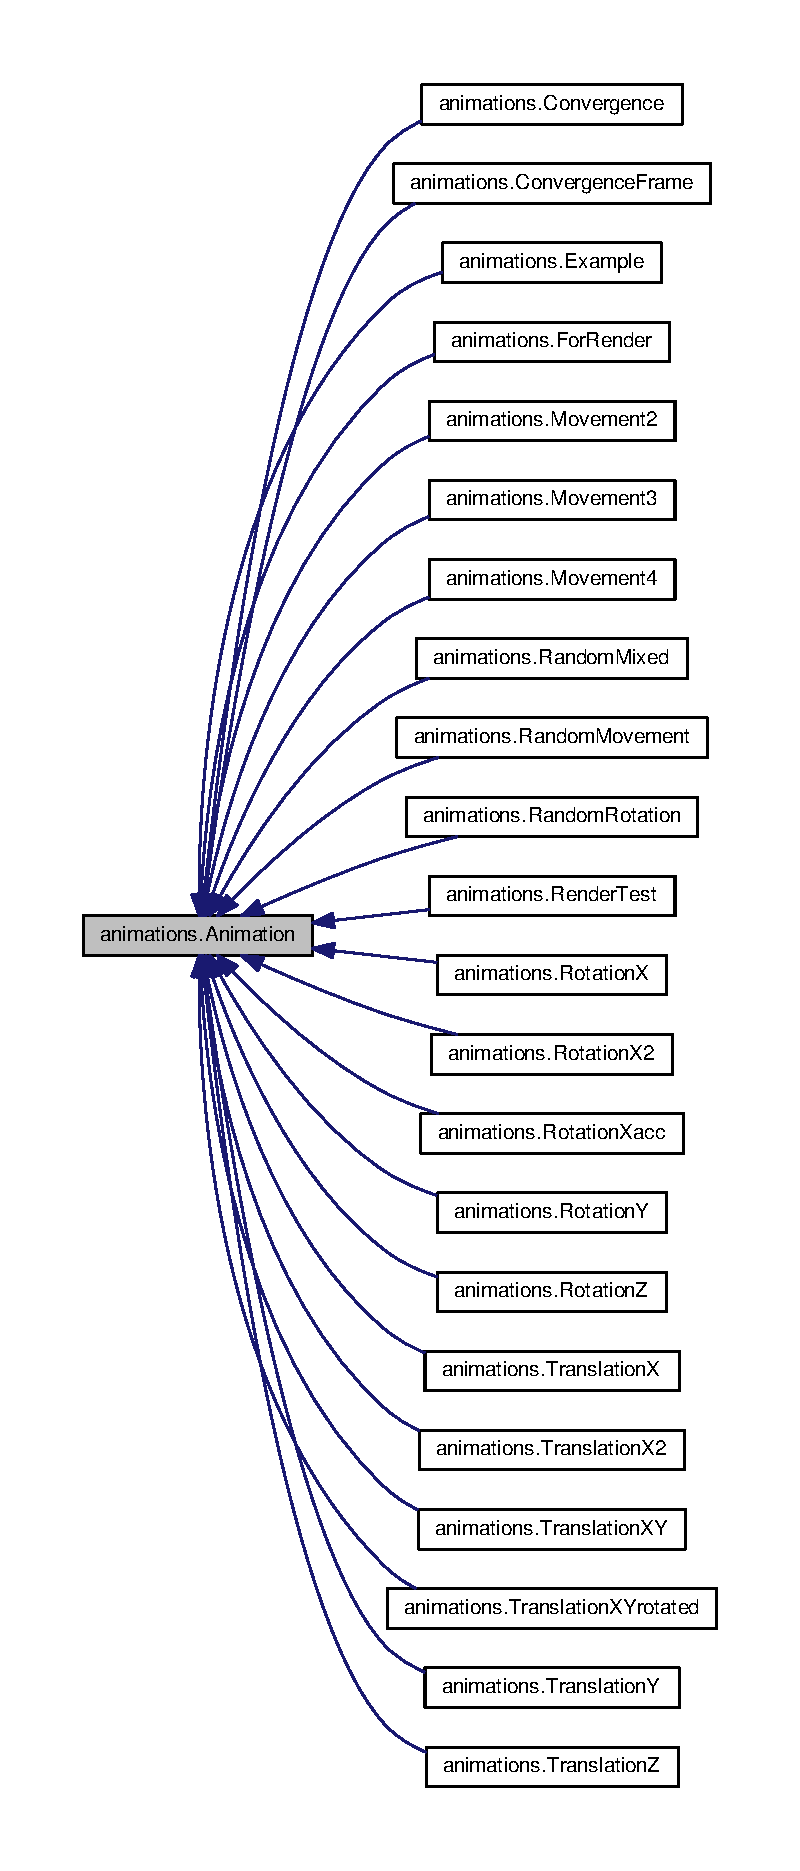
\includegraphics[height=550pt]{classanimations_1_1Animation__inherit__graph}
\end{center}
\end{figure}
\subsection*{Public Member Functions}
\begin{DoxyCompactItemize}
\item 
def \hyperlink{classanimations_1_1Animation_aecd6f3fd72fbe0cd9cdab02f51cedc70}{\+\_\+\+\_\+init\+\_\+\+\_\+} (self, bdr\+\_\+handler, blender\+\_\+object, frames)
\begin{DoxyCompactList}\small\item\em Creates new \hyperlink{classanimations_1_1Animation}{Animation}. \end{DoxyCompactList}\end{DoxyCompactItemize}
\subsection*{Static Public Member Functions}
\begin{DoxyCompactItemize}
\item 
def \hyperlink{classanimations_1_1Animation_aa74c4b0ca9995139e38353ae4ae99317}{get\+\_\+start\+\_\+position} ()\hypertarget{classanimations_1_1Animation_aa74c4b0ca9995139e38353ae4ae99317}{}\label{classanimations_1_1Animation_aa74c4b0ca9995139e38353ae4ae99317}

\begin{DoxyCompactList}\small\item\em Returns the init position. \end{DoxyCompactList}\item 
def \hyperlink{classanimations_1_1Animation_afb08c012c75c94c4bb01ea75c4df5dec}{get\+\_\+start\+\_\+rotation} ()\hypertarget{classanimations_1_1Animation_afb08c012c75c94c4bb01ea75c4df5dec}{}\label{classanimations_1_1Animation_afb08c012c75c94c4bb01ea75c4df5dec}

\begin{DoxyCompactList}\small\item\em Returns the init rotation. \end{DoxyCompactList}\end{DoxyCompactItemize}
\subsection*{Static Public Attributes}
\begin{DoxyCompactItemize}
\item 
{\bfseries obj} = None\hypertarget{classanimations_1_1Animation_ae67dfa9e3baa473cc672fa6a52f1cad5}{}\label{classanimations_1_1Animation_ae67dfa9e3baa473cc672fa6a52f1cad5}

\item 
string {\bfseries interpolation} = \char`\"{}Q\+U\+AD\char`\"{}\hypertarget{classanimations_1_1Animation_a6417103a8a9704bae9a9c97d87d862b4}{}\label{classanimations_1_1Animation_a6417103a8a9704bae9a9c97d87d862b4}

\end{DoxyCompactItemize}


\subsection{Constructor \& Destructor Documentation}
\index{animations\+::\+Animation@{animations\+::\+Animation}!\+\_\+\+\_\+init\+\_\+\+\_\+@{\+\_\+\+\_\+init\+\_\+\+\_\+}}
\index{\+\_\+\+\_\+init\+\_\+\+\_\+@{\+\_\+\+\_\+init\+\_\+\+\_\+}!animations\+::\+Animation@{animations\+::\+Animation}}
\subsubsection[{\texorpdfstring{\+\_\+\+\_\+init\+\_\+\+\_\+(self, bdr\+\_\+handler, blender\+\_\+object, frames)}{__init__(self, bdr_handler, blender_object, frames)}}]{\setlength{\rightskip}{0pt plus 5cm}def animations.\+Animation.\+\_\+\+\_\+init\+\_\+\+\_\+ (
\begin{DoxyParamCaption}
\item[{}]{self, }
\item[{}]{bdr\+\_\+handler, }
\item[{}]{blender\+\_\+object, }
\item[{}]{frames}
\end{DoxyParamCaption}
)}\hypertarget{classanimations_1_1Animation_aecd6f3fd72fbe0cd9cdab02f51cedc70}{}\label{classanimations_1_1Animation_aecd6f3fd72fbe0cd9cdab02f51cedc70}


Creates new \hyperlink{classanimations_1_1Animation}{Animation}. 

\hyperlink{classanimations_1_1Animation}{Animation} contains function for keyframe creation and initial pose. 
\begin{DoxyParams}{Parameters}
{\em bdr\+\_\+handler} & Blender\+Handler \\
\hline
{\em blender\+\_\+object} & Blender\+Object \\
\hline
{\em frames} & Number of frames the animation can use \\
\hline
\end{DoxyParams}


The documentation for this class was generated from the following file\+:\begin{DoxyCompactItemize}
\item 
/home/sebastian/catkin\+\_\+ws/src/animation\+\_\+render/scripts/framework/animations.\+py\end{DoxyCompactItemize}

\hypertarget{classAnimationRender}{}\section{Animation\+Render Class Reference}
\label{classAnimationRender}\index{Animation\+Render@{Animation\+Render}}
\subsection*{Public Member Functions}
\begin{DoxyCompactItemize}
\item 
\hyperlink{classAnimationRender_add45175c946790a10451ba9cdb5caa37}{Animation\+Render} (ros\+::\+Node\+Handle $\ast$nH)
\begin{DoxyCompactList}\small\item\em \hyperlink{classAnimationRender}{Animation\+Render} Constructor. \end{DoxyCompactList}\item 
void \hyperlink{classAnimationRender_a5badc5fbb7d9c2ce6f4f9b6dda610615}{start} ()\hypertarget{classAnimationRender_a5badc5fbb7d9c2ce6f4f9b6dda610615}{}\label{classAnimationRender_a5badc5fbb7d9c2ce6f4f9b6dda610615}

\begin{DoxyCompactList}\small\item\em start Start test procedure, is called by $<$\+Start\+Test$>$ command \end{DoxyCompactList}\item 
bool \hyperlink{classAnimationRender_ae21bd75361e818fd3c10c4b9a3def277}{download\+Template\+Image} ()
\begin{DoxyCompactList}\small\item\em Download current template image. \end{DoxyCompactList}\item 
bool \hyperlink{classAnimationRender_a2b6e770e27bb976e31e19a948fcce3af}{download\+Background\+Image} ()
\begin{DoxyCompactList}\small\item\em Dwonload current background image. \end{DoxyCompactList}\end{DoxyCompactItemize}


\subsection{Constructor \& Destructor Documentation}
\index{Animation\+Render@{Animation\+Render}!Animation\+Render@{Animation\+Render}}
\index{Animation\+Render@{Animation\+Render}!Animation\+Render@{Animation\+Render}}
\subsubsection[{\texorpdfstring{Animation\+Render(ros\+::\+Node\+Handle $\ast$n\+H)}{AnimationRender(ros::NodeHandle *nH)}}]{\setlength{\rightskip}{0pt plus 5cm}Animation\+Render\+::\+Animation\+Render (
\begin{DoxyParamCaption}
\item[{ros\+::\+Node\+Handle $\ast$}]{nH}
\end{DoxyParamCaption}
)}\hypertarget{classAnimationRender_add45175c946790a10451ba9cdb5caa37}{}\label{classAnimationRender_add45175c946790a10451ba9cdb5caa37}


\hyperlink{classAnimationRender}{Animation\+Render} Constructor. 


\begin{DoxyParams}{Parameters}
{\em nH} & \\
\hline
\end{DoxyParams}


\subsection{Member Function Documentation}
\index{Animation\+Render@{Animation\+Render}!download\+Background\+Image@{download\+Background\+Image}}
\index{download\+Background\+Image@{download\+Background\+Image}!Animation\+Render@{Animation\+Render}}
\subsubsection[{\texorpdfstring{download\+Background\+Image()}{downloadBackgroundImage()}}]{\setlength{\rightskip}{0pt plus 5cm}bool Animation\+Render\+::download\+Background\+Image (
\begin{DoxyParamCaption}
{}
\end{DoxyParamCaption}
)}\hypertarget{classAnimationRender_a2b6e770e27bb976e31e19a948fcce3af}{}\label{classAnimationRender_a2b6e770e27bb976e31e19a948fcce3af}


Dwonload current background image. 

\begin{DoxyReturn}{Returns}

\end{DoxyReturn}
\index{Animation\+Render@{Animation\+Render}!download\+Template\+Image@{download\+Template\+Image}}
\index{download\+Template\+Image@{download\+Template\+Image}!Animation\+Render@{Animation\+Render}}
\subsubsection[{\texorpdfstring{download\+Template\+Image()}{downloadTemplateImage()}}]{\setlength{\rightskip}{0pt plus 5cm}bool Animation\+Render\+::download\+Template\+Image (
\begin{DoxyParamCaption}
{}
\end{DoxyParamCaption}
)}\hypertarget{classAnimationRender_ae21bd75361e818fd3c10c4b9a3def277}{}\label{classAnimationRender_ae21bd75361e818fd3c10c4b9a3def277}


Download current template image. 

\begin{DoxyReturn}{Returns}

\end{DoxyReturn}


The documentation for this class was generated from the following files\+:\begin{DoxyCompactItemize}
\item 
/home/sebastian/catkin\+\_\+ws/src/animation\+\_\+render/src/animationrender.\+h\item 
/home/sebastian/catkin\+\_\+ws/src/animation\+\_\+render/src/animationrender.\+cpp\end{DoxyCompactItemize}

\hypertarget{classhandler_1_1BlenderHandler}{}\section{handler.\+Blender\+Handler Class Reference}
\label{classhandler_1_1BlenderHandler}\index{handler.\+Blender\+Handler@{handler.\+Blender\+Handler}}
\subsection*{Public Member Functions}
\begin{DoxyCompactItemize}
\item 
def \hyperlink{classhandler_1_1BlenderHandler_ab8b8c05e8cacd4deed51f02218ba75de}{\+\_\+\+\_\+init\+\_\+\+\_\+} (self, file\+\_\+path)
\begin{DoxyCompactList}\small\item\em Creates a new \hyperlink{classhandler_1_1BlenderHandler}{Blender\+Handler}. \end{DoxyCompactList}\item 
def \hyperlink{classhandler_1_1BlenderHandler_acf6429fb35078f4fb59510a46d5c80d1}{set\+\_\+background\+\_\+pil} (self, image)
\begin{DoxyCompactList}\small\item\em Set background image. \end{DoxyCompactList}\item 
def \hyperlink{classhandler_1_1BlenderHandler_a78adf542e7b1b6ffe009d680c01b2270}{set\+\_\+background} (self, image)
\begin{DoxyCompactList}\small\item\em Set background image. \end{DoxyCompactList}\item 
def \hyperlink{classhandler_1_1BlenderHandler_ae700e5cdd64c7efc38fd704c382de27d}{set\+\_\+horizon\+\_\+color} (self, color)
\begin{DoxyCompactList}\small\item\em Set horizon color. \end{DoxyCompactList}\item 
def \hyperlink{classhandler_1_1BlenderHandler_a73b1060e394c8f36355e7bdcf126eb6e}{use\+\_\+anti\+\_\+aliasing} (self, b)
\begin{DoxyCompactList}\small\item\em Enable or disable anti aliasing. \end{DoxyCompactList}\item 
def \hyperlink{classhandler_1_1BlenderHandler_aa4978ad675a1c206fddae198ef445d60}{set\+\_\+fps} (self, fps)
\begin{DoxyCompactList}\small\item\em Set frame per second of rendered video. \end{DoxyCompactList}\item 
def \hyperlink{classhandler_1_1BlenderHandler_a9bacab8f5968c9d8611ca3f138a07d44}{set\+\_\+focal\+\_\+length} (self, focal\+\_\+length)
\begin{DoxyCompactList}\small\item\em Set focal length of camera. \end{DoxyCompactList}\item 
def \hyperlink{classhandler_1_1BlenderHandler_a3cc2cb039094ea02c6eda160d1240222}{set\+\_\+sensor\+\_\+width} (self, sensor\+\_\+width)
\begin{DoxyCompactList}\small\item\em Set sensor width of camera. \end{DoxyCompactList}\item 
def \hyperlink{classhandler_1_1BlenderHandler_af139c2e779c27473a4b85358b5df86c9}{set\+\_\+interpolation} (self, interpol)
\begin{DoxyCompactList}\small\item\em Set interpolation modus between keyframes. \end{DoxyCompactList}\item 
def \hyperlink{classhandler_1_1BlenderHandler_ae5e76e83e09fc173400b8c393ef27104}{use\+\_\+environment\+\_\+light} (self, b)
\begin{DoxyCompactList}\small\item\em Enable or disable environmental lighting. \end{DoxyCompactList}\item 
def \hyperlink{classhandler_1_1BlenderHandler_acf1f1e79abdcfb407510e429bc31149c}{set\+\_\+environment\+\_\+energy} (self, e)
\begin{DoxyCompactList}\small\item\em Set enegery of environmental lighting. \end{DoxyCompactList}\item 
def \hyperlink{classhandler_1_1BlenderHandler_a95d530555428c5af8106d18a34cd3721}{render\+\_\+and\+\_\+save} (self, path=None)
\begin{DoxyCompactList}\small\item\em Render current image and save it. \end{DoxyCompactList}\item 
def \hyperlink{classhandler_1_1BlenderHandler_a5fbc1bc58986c32ee7dedbc67cd3dcbe}{animation\+\_\+and\+\_\+save} (self, path=None)
\begin{DoxyCompactList}\small\item\em Render video and save it. \end{DoxyCompactList}\end{DoxyCompactItemize}
\subsection*{Static Public Member Functions}
\begin{DoxyCompactItemize}
\item 
def \hyperlink{classhandler_1_1BlenderHandler_aaf2a3e4a6e5ecd003415d5543143767e}{set\+\_\+resolution} (x, y)
\begin{DoxyCompactList}\small\item\em Set resolution of rendered image or video. \end{DoxyCompactList}\end{DoxyCompactItemize}
\subsection*{Static Public Attributes}
\begin{DoxyCompactItemize}
\item 
{\bfseries file\+\_\+path} = None\hypertarget{classhandler_1_1BlenderHandler_ab4129f1d57bcef67c29f9959b690f890}{}\label{classhandler_1_1BlenderHandler_ab4129f1d57bcef67c29f9959b690f890}

\item 
{\bfseries world} = None\hypertarget{classhandler_1_1BlenderHandler_a6ed4f22d3f26a59dc74cea2bdd7669f3}{}\label{classhandler_1_1BlenderHandler_a6ed4f22d3f26a59dc74cea2bdd7669f3}

\item 
{\bfseries scene} = None\hypertarget{classhandler_1_1BlenderHandler_a71ab33d3e6cbfa1ecd5fa8b3bb57b4e0}{}\label{classhandler_1_1BlenderHandler_a71ab33d3e6cbfa1ecd5fa8b3bb57b4e0}

\item 
{\bfseries camera} = None\hypertarget{classhandler_1_1BlenderHandler_aa8b6ac7800ecf397f96f6c520391ec89}{}\label{classhandler_1_1BlenderHandler_aa8b6ac7800ecf397f96f6c520391ec89}

\item 
{\bfseries bgr\+\_\+img} = None\hypertarget{classhandler_1_1BlenderHandler_a40868d51142328068c0b060ca59761b4}{}\label{classhandler_1_1BlenderHandler_a40868d51142328068c0b060ca59761b4}

\item 
{\bfseries bgr\+\_\+tex} = None\hypertarget{classhandler_1_1BlenderHandler_a4893c39b2c6609495464c6fe04c476cf}{}\label{classhandler_1_1BlenderHandler_a4893c39b2c6609495464c6fe04c476cf}

\item 
{\bfseries bgr\+\_\+tex\+\_\+slot} = None\hypertarget{classhandler_1_1BlenderHandler_a9c268946601a4973309ac2a03dcb57c9}{}\label{classhandler_1_1BlenderHandler_a9c268946601a4973309ac2a03dcb57c9}

\end{DoxyCompactItemize}


\subsection{Constructor \& Destructor Documentation}
\index{handler\+::\+Blender\+Handler@{handler\+::\+Blender\+Handler}!\+\_\+\+\_\+init\+\_\+\+\_\+@{\+\_\+\+\_\+init\+\_\+\+\_\+}}
\index{\+\_\+\+\_\+init\+\_\+\+\_\+@{\+\_\+\+\_\+init\+\_\+\+\_\+}!handler\+::\+Blender\+Handler@{handler\+::\+Blender\+Handler}}
\subsubsection[{\texorpdfstring{\+\_\+\+\_\+init\+\_\+\+\_\+(self, file\+\_\+path)}{__init__(self, file_path)}}]{\setlength{\rightskip}{0pt plus 5cm}def handler.\+Blender\+Handler.\+\_\+\+\_\+init\+\_\+\+\_\+ (
\begin{DoxyParamCaption}
\item[{}]{self, }
\item[{}]{file\+\_\+path}
\end{DoxyParamCaption}
)}\hypertarget{classhandler_1_1BlenderHandler_ab8b8c05e8cacd4deed51f02218ba75de}{}\label{classhandler_1_1BlenderHandler_ab8b8c05e8cacd4deed51f02218ba75de}


Creates a new \hyperlink{classhandler_1_1BlenderHandler}{Blender\+Handler}. 

This class contains all important functions and objects of blender.


\begin{DoxyParams}{Parameters}
{\em file\+\_\+path} & Output path for rendered images and videos \\
\hline
\end{DoxyParams}


\subsection{Member Function Documentation}
\index{handler\+::\+Blender\+Handler@{handler\+::\+Blender\+Handler}!animation\+\_\+and\+\_\+save@{animation\+\_\+and\+\_\+save}}
\index{animation\+\_\+and\+\_\+save@{animation\+\_\+and\+\_\+save}!handler\+::\+Blender\+Handler@{handler\+::\+Blender\+Handler}}
\subsubsection[{\texorpdfstring{animation\+\_\+and\+\_\+save(self, path=\+None)}{animation_and_save(self, path=None)}}]{\setlength{\rightskip}{0pt plus 5cm}def handler.\+Blender\+Handler.\+animation\+\_\+and\+\_\+save (
\begin{DoxyParamCaption}
\item[{}]{self, }
\item[{}]{path = {\ttfamily None}}
\end{DoxyParamCaption}
)}\hypertarget{classhandler_1_1BlenderHandler_a5fbc1bc58986c32ee7dedbc67cd3dcbe}{}\label{classhandler_1_1BlenderHandler_a5fbc1bc58986c32ee7dedbc67cd3dcbe}


Render video and save it. 


\begin{DoxyParams}{Parameters}
{\em path} & Output path. If None, file\+\_\+path is used. \\
\hline
\end{DoxyParams}
\index{handler\+::\+Blender\+Handler@{handler\+::\+Blender\+Handler}!render\+\_\+and\+\_\+save@{render\+\_\+and\+\_\+save}}
\index{render\+\_\+and\+\_\+save@{render\+\_\+and\+\_\+save}!handler\+::\+Blender\+Handler@{handler\+::\+Blender\+Handler}}
\subsubsection[{\texorpdfstring{render\+\_\+and\+\_\+save(self, path=\+None)}{render_and_save(self, path=None)}}]{\setlength{\rightskip}{0pt plus 5cm}def handler.\+Blender\+Handler.\+render\+\_\+and\+\_\+save (
\begin{DoxyParamCaption}
\item[{}]{self, }
\item[{}]{path = {\ttfamily None}}
\end{DoxyParamCaption}
)}\hypertarget{classhandler_1_1BlenderHandler_a95d530555428c5af8106d18a34cd3721}{}\label{classhandler_1_1BlenderHandler_a95d530555428c5af8106d18a34cd3721}


Render current image and save it. 


\begin{DoxyParams}{Parameters}
{\em path} & Output path. If None, file\+\_\+path is used. \\
\hline
\end{DoxyParams}
\index{handler\+::\+Blender\+Handler@{handler\+::\+Blender\+Handler}!set\+\_\+background@{set\+\_\+background}}
\index{set\+\_\+background@{set\+\_\+background}!handler\+::\+Blender\+Handler@{handler\+::\+Blender\+Handler}}
\subsubsection[{\texorpdfstring{set\+\_\+background(self, image)}{set_background(self, image)}}]{\setlength{\rightskip}{0pt plus 5cm}def handler.\+Blender\+Handler.\+set\+\_\+background (
\begin{DoxyParamCaption}
\item[{}]{self, }
\item[{}]{image}
\end{DoxyParamCaption}
)}\hypertarget{classhandler_1_1BlenderHandler_a78adf542e7b1b6ffe009d680c01b2270}{}\label{classhandler_1_1BlenderHandler_a78adf542e7b1b6ffe009d680c01b2270}


Set background image. 


\begin{DoxyParams}{Parameters}
{\em image} & Image path \\
\hline
\end{DoxyParams}
\index{handler\+::\+Blender\+Handler@{handler\+::\+Blender\+Handler}!set\+\_\+background\+\_\+pil@{set\+\_\+background\+\_\+pil}}
\index{set\+\_\+background\+\_\+pil@{set\+\_\+background\+\_\+pil}!handler\+::\+Blender\+Handler@{handler\+::\+Blender\+Handler}}
\subsubsection[{\texorpdfstring{set\+\_\+background\+\_\+pil(self, image)}{set_background_pil(self, image)}}]{\setlength{\rightskip}{0pt plus 5cm}def handler.\+Blender\+Handler.\+set\+\_\+background\+\_\+pil (
\begin{DoxyParamCaption}
\item[{}]{self, }
\item[{}]{image}
\end{DoxyParamCaption}
)}\hypertarget{classhandler_1_1BlenderHandler_acf6429fb35078f4fb59510a46d5c80d1}{}\label{classhandler_1_1BlenderHandler_acf6429fb35078f4fb59510a46d5c80d1}


Set background image. 


\begin{DoxyParams}{Parameters}
{\em image} & P\+IL image \\
\hline
\end{DoxyParams}
\index{handler\+::\+Blender\+Handler@{handler\+::\+Blender\+Handler}!set\+\_\+environment\+\_\+energy@{set\+\_\+environment\+\_\+energy}}
\index{set\+\_\+environment\+\_\+energy@{set\+\_\+environment\+\_\+energy}!handler\+::\+Blender\+Handler@{handler\+::\+Blender\+Handler}}
\subsubsection[{\texorpdfstring{set\+\_\+environment\+\_\+energy(self, e)}{set_environment_energy(self, e)}}]{\setlength{\rightskip}{0pt plus 5cm}def handler.\+Blender\+Handler.\+set\+\_\+environment\+\_\+energy (
\begin{DoxyParamCaption}
\item[{}]{self, }
\item[{}]{e}
\end{DoxyParamCaption}
)}\hypertarget{classhandler_1_1BlenderHandler_acf1f1e79abdcfb407510e429bc31149c}{}\label{classhandler_1_1BlenderHandler_acf1f1e79abdcfb407510e429bc31149c}


Set enegery of environmental lighting. 

Only necessary if enabled. 
\begin{DoxyParams}{Parameters}
{\em e} & Energy \\
\hline
\end{DoxyParams}
\index{handler\+::\+Blender\+Handler@{handler\+::\+Blender\+Handler}!set\+\_\+focal\+\_\+length@{set\+\_\+focal\+\_\+length}}
\index{set\+\_\+focal\+\_\+length@{set\+\_\+focal\+\_\+length}!handler\+::\+Blender\+Handler@{handler\+::\+Blender\+Handler}}
\subsubsection[{\texorpdfstring{set\+\_\+focal\+\_\+length(self, focal\+\_\+length)}{set_focal_length(self, focal_length)}}]{\setlength{\rightskip}{0pt plus 5cm}def handler.\+Blender\+Handler.\+set\+\_\+focal\+\_\+length (
\begin{DoxyParamCaption}
\item[{}]{self, }
\item[{}]{focal\+\_\+length}
\end{DoxyParamCaption}
)}\hypertarget{classhandler_1_1BlenderHandler_a9bacab8f5968c9d8611ca3f138a07d44}{}\label{classhandler_1_1BlenderHandler_a9bacab8f5968c9d8611ca3f138a07d44}


Set focal length of camera. 


\begin{DoxyParams}{Parameters}
{\em focal\+\_\+length} & Focal length in mm \\
\hline
\end{DoxyParams}
\index{handler\+::\+Blender\+Handler@{handler\+::\+Blender\+Handler}!set\+\_\+fps@{set\+\_\+fps}}
\index{set\+\_\+fps@{set\+\_\+fps}!handler\+::\+Blender\+Handler@{handler\+::\+Blender\+Handler}}
\subsubsection[{\texorpdfstring{set\+\_\+fps(self, fps)}{set_fps(self, fps)}}]{\setlength{\rightskip}{0pt plus 5cm}def handler.\+Blender\+Handler.\+set\+\_\+fps (
\begin{DoxyParamCaption}
\item[{}]{self, }
\item[{}]{fps}
\end{DoxyParamCaption}
)}\hypertarget{classhandler_1_1BlenderHandler_aa4978ad675a1c206fddae198ef445d60}{}\label{classhandler_1_1BlenderHandler_aa4978ad675a1c206fddae198ef445d60}


Set frame per second of rendered video. 


\begin{DoxyParams}{Parameters}
{\em fps} & Frames per second \\
\hline
\end{DoxyParams}
\index{handler\+::\+Blender\+Handler@{handler\+::\+Blender\+Handler}!set\+\_\+horizon\+\_\+color@{set\+\_\+horizon\+\_\+color}}
\index{set\+\_\+horizon\+\_\+color@{set\+\_\+horizon\+\_\+color}!handler\+::\+Blender\+Handler@{handler\+::\+Blender\+Handler}}
\subsubsection[{\texorpdfstring{set\+\_\+horizon\+\_\+color(self, color)}{set_horizon_color(self, color)}}]{\setlength{\rightskip}{0pt plus 5cm}def handler.\+Blender\+Handler.\+set\+\_\+horizon\+\_\+color (
\begin{DoxyParamCaption}
\item[{}]{self, }
\item[{}]{color}
\end{DoxyParamCaption}
)}\hypertarget{classhandler_1_1BlenderHandler_ae700e5cdd64c7efc38fd704c382de27d}{}\label{classhandler_1_1BlenderHandler_ae700e5cdd64c7efc38fd704c382de27d}


Set horizon color. 


\begin{DoxyParams}{Parameters}
{\em color} & Color in R\+GB \\
\hline
\end{DoxyParams}
\index{handler\+::\+Blender\+Handler@{handler\+::\+Blender\+Handler}!set\+\_\+interpolation@{set\+\_\+interpolation}}
\index{set\+\_\+interpolation@{set\+\_\+interpolation}!handler\+::\+Blender\+Handler@{handler\+::\+Blender\+Handler}}
\subsubsection[{\texorpdfstring{set\+\_\+interpolation(self, interpol)}{set_interpolation(self, interpol)}}]{\setlength{\rightskip}{0pt plus 5cm}def handler.\+Blender\+Handler.\+set\+\_\+interpolation (
\begin{DoxyParamCaption}
\item[{}]{self, }
\item[{}]{interpol}
\end{DoxyParamCaption}
)}\hypertarget{classhandler_1_1BlenderHandler_af139c2e779c27473a4b85358b5df86c9}{}\label{classhandler_1_1BlenderHandler_af139c2e779c27473a4b85358b5df86c9}


Set interpolation modus between keyframes. 

Can be set in the Animation 
\begin{DoxyParams}{Parameters}
{\em interpol} & Interpolation modus. For example\+: \char`\"{}\+L\+I\+N\+E\+A\+R\char`\"{}, \char`\"{}\+B\+E\+Z\+I\+E\+R\char`\"{}, \char`\"{}\+Q\+U\+A\+D\char`\"{} \\
\hline
\end{DoxyParams}
\index{handler\+::\+Blender\+Handler@{handler\+::\+Blender\+Handler}!set\+\_\+resolution@{set\+\_\+resolution}}
\index{set\+\_\+resolution@{set\+\_\+resolution}!handler\+::\+Blender\+Handler@{handler\+::\+Blender\+Handler}}
\subsubsection[{\texorpdfstring{set\+\_\+resolution(x, y)}{set_resolution(x, y)}}]{\setlength{\rightskip}{0pt plus 5cm}def handler.\+Blender\+Handler.\+set\+\_\+resolution (
\begin{DoxyParamCaption}
\item[{}]{x, }
\item[{}]{y}
\end{DoxyParamCaption}
)\hspace{0.3cm}{\ttfamily [static]}}\hypertarget{classhandler_1_1BlenderHandler_aaf2a3e4a6e5ecd003415d5543143767e}{}\label{classhandler_1_1BlenderHandler_aaf2a3e4a6e5ecd003415d5543143767e}


Set resolution of rendered image or video. 


\begin{DoxyParams}{Parameters}
{\em x} & width in pixel \\
\hline
{\em y} & height in pixel \\
\hline
\end{DoxyParams}
\index{handler\+::\+Blender\+Handler@{handler\+::\+Blender\+Handler}!set\+\_\+sensor\+\_\+width@{set\+\_\+sensor\+\_\+width}}
\index{set\+\_\+sensor\+\_\+width@{set\+\_\+sensor\+\_\+width}!handler\+::\+Blender\+Handler@{handler\+::\+Blender\+Handler}}
\subsubsection[{\texorpdfstring{set\+\_\+sensor\+\_\+width(self, sensor\+\_\+width)}{set_sensor_width(self, sensor_width)}}]{\setlength{\rightskip}{0pt plus 5cm}def handler.\+Blender\+Handler.\+set\+\_\+sensor\+\_\+width (
\begin{DoxyParamCaption}
\item[{}]{self, }
\item[{}]{sensor\+\_\+width}
\end{DoxyParamCaption}
)}\hypertarget{classhandler_1_1BlenderHandler_a3cc2cb039094ea02c6eda160d1240222}{}\label{classhandler_1_1BlenderHandler_a3cc2cb039094ea02c6eda160d1240222}


Set sensor width of camera. 


\begin{DoxyParams}{Parameters}
{\em sensor\+\_\+width} & Sensor width in mm \\
\hline
\end{DoxyParams}
\index{handler\+::\+Blender\+Handler@{handler\+::\+Blender\+Handler}!use\+\_\+anti\+\_\+aliasing@{use\+\_\+anti\+\_\+aliasing}}
\index{use\+\_\+anti\+\_\+aliasing@{use\+\_\+anti\+\_\+aliasing}!handler\+::\+Blender\+Handler@{handler\+::\+Blender\+Handler}}
\subsubsection[{\texorpdfstring{use\+\_\+anti\+\_\+aliasing(self, b)}{use_anti_aliasing(self, b)}}]{\setlength{\rightskip}{0pt plus 5cm}def handler.\+Blender\+Handler.\+use\+\_\+anti\+\_\+aliasing (
\begin{DoxyParamCaption}
\item[{}]{self, }
\item[{}]{b}
\end{DoxyParamCaption}
)}\hypertarget{classhandler_1_1BlenderHandler_a73b1060e394c8f36355e7bdcf126eb6e}{}\label{classhandler_1_1BlenderHandler_a73b1060e394c8f36355e7bdcf126eb6e}


Enable or disable anti aliasing. 


\begin{DoxyParams}{Parameters}
{\em b} & True\+: Enable, False\+: Disable \\
\hline
\end{DoxyParams}
\index{handler\+::\+Blender\+Handler@{handler\+::\+Blender\+Handler}!use\+\_\+environment\+\_\+light@{use\+\_\+environment\+\_\+light}}
\index{use\+\_\+environment\+\_\+light@{use\+\_\+environment\+\_\+light}!handler\+::\+Blender\+Handler@{handler\+::\+Blender\+Handler}}
\subsubsection[{\texorpdfstring{use\+\_\+environment\+\_\+light(self, b)}{use_environment_light(self, b)}}]{\setlength{\rightskip}{0pt plus 5cm}def handler.\+Blender\+Handler.\+use\+\_\+environment\+\_\+light (
\begin{DoxyParamCaption}
\item[{}]{self, }
\item[{}]{b}
\end{DoxyParamCaption}
)}\hypertarget{classhandler_1_1BlenderHandler_ae5e76e83e09fc173400b8c393ef27104}{}\label{classhandler_1_1BlenderHandler_ae5e76e83e09fc173400b8c393ef27104}


Enable or disable environmental lighting. 


\begin{DoxyParams}{Parameters}
{\em b} & True\+: Enable, False\+: Disable \\
\hline
\end{DoxyParams}


The documentation for this class was generated from the following file\+:\begin{DoxyCompactItemize}
\item 
/home/sebastian/catkin\+\_\+ws/src/animation\+\_\+render/scripts/framework/handler.\+py\end{DoxyCompactItemize}

\hypertarget{classobjects_1_1BlenderObject}{}\section{objects.\+Blender\+Object Class Reference}
\label{classobjects_1_1BlenderObject}\index{objects.\+Blender\+Object@{objects.\+Blender\+Object}}


Inheritance diagram for objects.\+Blender\+Object\+:\nopagebreak
\begin{figure}[H]
\begin{center}
\leavevmode
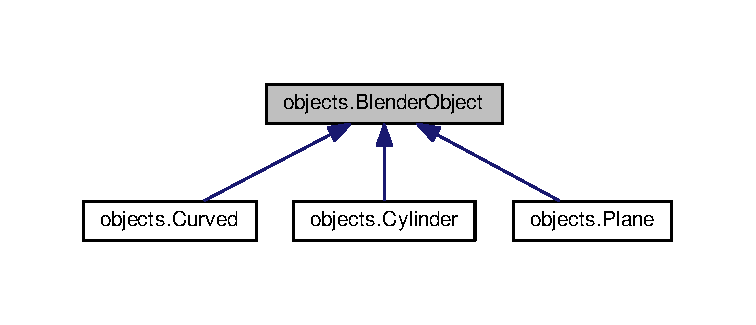
\includegraphics[width=350pt]{classobjects_1_1BlenderObject__inherit__graph}
\end{center}
\end{figure}
\subsection*{Public Member Functions}
\begin{DoxyCompactItemize}
\item 
def {\bfseries \+\_\+\+\_\+init\+\_\+\+\_\+} (self, name, image=None)\hypertarget{classobjects_1_1BlenderObject_a53848afaa4520cb9a4829a3195431305}{}\label{classobjects_1_1BlenderObject_a53848afaa4520cb9a4829a3195431305}

\item 
def \hyperlink{classobjects_1_1BlenderObject_a1fba576cf5d5e0da4e6e4bf527910d9a}{set\+\_\+location} (self, loc)
\begin{DoxyCompactList}\small\item\em Set location of the object. \end{DoxyCompactList}\item 
def \hyperlink{classobjects_1_1BlenderObject_a2cb1f87c44cc7679e22ec411d731f9c1}{set\+\_\+rotation} (self, rot)
\begin{DoxyCompactList}\small\item\em Set rotation of the object. \end{DoxyCompactList}\item 
def \hyperlink{classobjects_1_1BlenderObject_a6867acef4c79697a549e7420f1365528}{set\+\_\+image} (self, image)
\begin{DoxyCompactList}\small\item\em Set template image of the object. \end{DoxyCompactList}\item 
def \hyperlink{classobjects_1_1BlenderObject_aa9e2a9a207bd727c7ee942dae6c78454}{keyframe\+\_\+insert} (self, keyframe\+\_\+type, frame)
\begin{DoxyCompactList}\small\item\em Insert key frame. \end{DoxyCompactList}\end{DoxyCompactItemize}
\subsection*{Static Public Attributes}
\begin{DoxyCompactItemize}
\item 
{\bfseries name} = None\hypertarget{classobjects_1_1BlenderObject_adde52beb662c2c048be25e6d1ebcffed}{}\label{classobjects_1_1BlenderObject_adde52beb662c2c048be25e6d1ebcffed}

\item 
{\bfseries obj} = None\hypertarget{classobjects_1_1BlenderObject_a167aa00bad9fa6c397376abe59082924}{}\label{classobjects_1_1BlenderObject_a167aa00bad9fa6c397376abe59082924}

\item 
{\bfseries img} = None\hypertarget{classobjects_1_1BlenderObject_ab70c76e6c64e8fdedb8794aabfd3c769}{}\label{classobjects_1_1BlenderObject_ab70c76e6c64e8fdedb8794aabfd3c769}

\item 
{\bfseries tex} = None\hypertarget{classobjects_1_1BlenderObject_ad31e2cfb187de50cb1fe7a52ba844600}{}\label{classobjects_1_1BlenderObject_ad31e2cfb187de50cb1fe7a52ba844600}

\item 
{\bfseries mat} = None\hypertarget{classobjects_1_1BlenderObject_a926b93366f3f14f20254ad181bdd60c5}{}\label{classobjects_1_1BlenderObject_a926b93366f3f14f20254ad181bdd60c5}

\end{DoxyCompactItemize}


\subsection{Member Function Documentation}
\index{objects\+::\+Blender\+Object@{objects\+::\+Blender\+Object}!keyframe\+\_\+insert@{keyframe\+\_\+insert}}
\index{keyframe\+\_\+insert@{keyframe\+\_\+insert}!objects\+::\+Blender\+Object@{objects\+::\+Blender\+Object}}
\subsubsection[{\texorpdfstring{keyframe\+\_\+insert(self, keyframe\+\_\+type, frame)}{keyframe_insert(self, keyframe_type, frame)}}]{\setlength{\rightskip}{0pt plus 5cm}def objects.\+Blender\+Object.\+keyframe\+\_\+insert (
\begin{DoxyParamCaption}
\item[{}]{self, }
\item[{}]{keyframe\+\_\+type, }
\item[{}]{frame}
\end{DoxyParamCaption}
)}\hypertarget{classobjects_1_1BlenderObject_aa9e2a9a207bd727c7ee942dae6c78454}{}\label{classobjects_1_1BlenderObject_aa9e2a9a207bd727c7ee942dae6c78454}


Insert key frame. 


\begin{DoxyParams}{Parameters}
{\em keyframe\+\_\+type} & \textquotesingle{}rotation\+\_\+euler\textquotesingle{}, \textquotesingle{}location\textquotesingle{} \\
\hline
{\em frame} & Frame number \\
\hline
\end{DoxyParams}
\index{objects\+::\+Blender\+Object@{objects\+::\+Blender\+Object}!set\+\_\+image@{set\+\_\+image}}
\index{set\+\_\+image@{set\+\_\+image}!objects\+::\+Blender\+Object@{objects\+::\+Blender\+Object}}
\subsubsection[{\texorpdfstring{set\+\_\+image(self, image)}{set_image(self, image)}}]{\setlength{\rightskip}{0pt plus 5cm}def objects.\+Blender\+Object.\+set\+\_\+image (
\begin{DoxyParamCaption}
\item[{}]{self, }
\item[{}]{image}
\end{DoxyParamCaption}
)}\hypertarget{classobjects_1_1BlenderObject_a6867acef4c79697a549e7420f1365528}{}\label{classobjects_1_1BlenderObject_a6867acef4c79697a549e7420f1365528}


Set template image of the object. 


\begin{DoxyParams}{Parameters}
{\em image} & Template image \\
\hline
\end{DoxyParams}
\index{objects\+::\+Blender\+Object@{objects\+::\+Blender\+Object}!set\+\_\+location@{set\+\_\+location}}
\index{set\+\_\+location@{set\+\_\+location}!objects\+::\+Blender\+Object@{objects\+::\+Blender\+Object}}
\subsubsection[{\texorpdfstring{set\+\_\+location(self, loc)}{set_location(self, loc)}}]{\setlength{\rightskip}{0pt plus 5cm}def objects.\+Blender\+Object.\+set\+\_\+location (
\begin{DoxyParamCaption}
\item[{}]{self, }
\item[{}]{loc}
\end{DoxyParamCaption}
)}\hypertarget{classobjects_1_1BlenderObject_a1fba576cf5d5e0da4e6e4bf527910d9a}{}\label{classobjects_1_1BlenderObject_a1fba576cf5d5e0da4e6e4bf527910d9a}


Set location of the object. 


\begin{DoxyParams}{Parameters}
{\em loc} & Location \\
\hline
\end{DoxyParams}
\index{objects\+::\+Blender\+Object@{objects\+::\+Blender\+Object}!set\+\_\+rotation@{set\+\_\+rotation}}
\index{set\+\_\+rotation@{set\+\_\+rotation}!objects\+::\+Blender\+Object@{objects\+::\+Blender\+Object}}
\subsubsection[{\texorpdfstring{set\+\_\+rotation(self, rot)}{set_rotation(self, rot)}}]{\setlength{\rightskip}{0pt plus 5cm}def objects.\+Blender\+Object.\+set\+\_\+rotation (
\begin{DoxyParamCaption}
\item[{}]{self, }
\item[{}]{rot}
\end{DoxyParamCaption}
)}\hypertarget{classobjects_1_1BlenderObject_a2cb1f87c44cc7679e22ec411d731f9c1}{}\label{classobjects_1_1BlenderObject_a2cb1f87c44cc7679e22ec411d731f9c1}


Set rotation of the object. 


\begin{DoxyParams}{Parameters}
{\em rot} & rotation \\
\hline
\end{DoxyParams}


The documentation for this class was generated from the following file\+:\begin{DoxyCompactItemize}
\item 
/home/sebastian/catkin\+\_\+ws/src/animation\+\_\+render/scripts/framework/objects.\+py\end{DoxyCompactItemize}

\hypertarget{classanimations_1_1Convergence}{}\section{animations.\+Convergence Class Reference}
\label{classanimations_1_1Convergence}\index{animations.\+Convergence@{animations.\+Convergence}}


Inheritance diagram for animations.\+Convergence\+:\nopagebreak
\begin{figure}[H]
\begin{center}
\leavevmode
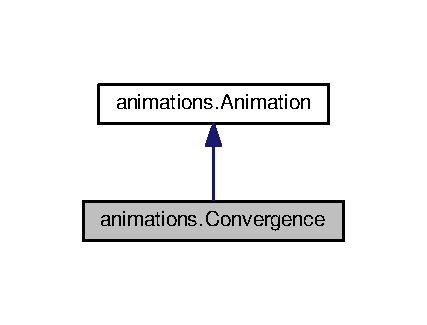
\includegraphics[width=205pt]{classanimations_1_1Convergence__inherit__graph}
\end{center}
\end{figure}


Collaboration diagram for animations.\+Convergence\+:\nopagebreak
\begin{figure}[H]
\begin{center}
\leavevmode
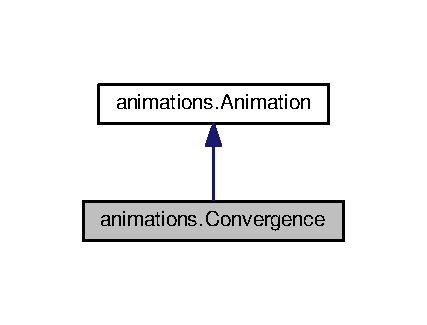
\includegraphics[width=205pt]{classanimations_1_1Convergence__coll__graph}
\end{center}
\end{figure}
\subsection*{Public Member Functions}
\begin{DoxyCompactItemize}
\item 
def {\bfseries \+\_\+\+\_\+init\+\_\+\+\_\+} (self, bdr\+\_\+handler, blender\+\_\+object, frames)\hypertarget{classanimations_1_1Convergence_a33c1c9719ce9ac7a75d3037b452927b3}{}\label{classanimations_1_1Convergence_a33c1c9719ce9ac7a75d3037b452927b3}

\end{DoxyCompactItemize}
\subsection*{Static Public Member Functions}
\begin{DoxyCompactItemize}
\item 
def {\bfseries get\+\_\+start\+\_\+position} ()\hypertarget{classanimations_1_1Convergence_a64c5262263dc44ef5ed4e4bb7d4a5f5a}{}\label{classanimations_1_1Convergence_a64c5262263dc44ef5ed4e4bb7d4a5f5a}

\item 
def {\bfseries get\+\_\+start\+\_\+rotation} ()\hypertarget{classanimations_1_1Convergence_a4d0adad10da4f7787cdcdf0eea6e92ed}{}\label{classanimations_1_1Convergence_a4d0adad10da4f7787cdcdf0eea6e92ed}

\end{DoxyCompactItemize}
\subsection*{Additional Inherited Members}


The documentation for this class was generated from the following file\+:\begin{DoxyCompactItemize}
\item 
/home/sebastian/catkin\+\_\+ws/src/animation\+\_\+render/scripts/framework/animations.\+py\end{DoxyCompactItemize}

\hypertarget{classanimations_1_1ConvergenceFrame}{}\section{animations.\+Convergence\+Frame Class Reference}
\label{classanimations_1_1ConvergenceFrame}\index{animations.\+Convergence\+Frame@{animations.\+Convergence\+Frame}}


Inheritance diagram for animations.\+Convergence\+Frame\+:\nopagebreak
\begin{figure}[H]
\begin{center}
\leavevmode
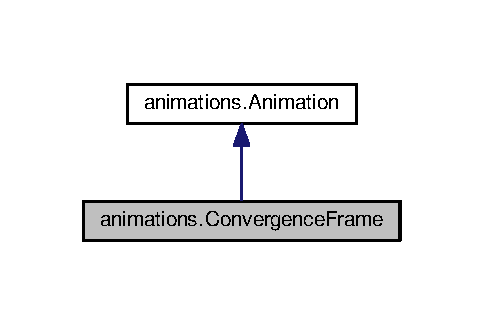
\includegraphics[width=232pt]{classanimations_1_1ConvergenceFrame__inherit__graph}
\end{center}
\end{figure}


Collaboration diagram for animations.\+Convergence\+Frame\+:\nopagebreak
\begin{figure}[H]
\begin{center}
\leavevmode
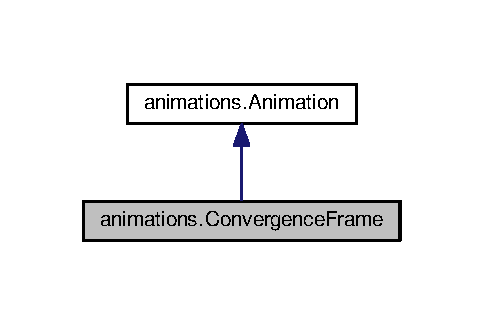
\includegraphics[width=232pt]{classanimations_1_1ConvergenceFrame__coll__graph}
\end{center}
\end{figure}
\subsection*{Public Member Functions}
\begin{DoxyCompactItemize}
\item 
def {\bfseries \+\_\+\+\_\+init\+\_\+\+\_\+} (self, bdr\+\_\+handler, blender\+\_\+object, frames)\hypertarget{classanimations_1_1ConvergenceFrame_a8c311e0e9fff583b2cfb7edeee0768ac}{}\label{classanimations_1_1ConvergenceFrame_a8c311e0e9fff583b2cfb7edeee0768ac}

\end{DoxyCompactItemize}
\subsection*{Static Public Member Functions}
\begin{DoxyCompactItemize}
\item 
def {\bfseries get\+\_\+start\+\_\+position} ()\hypertarget{classanimations_1_1ConvergenceFrame_ab8a836c49f3ff61e78acf3858a736fa9}{}\label{classanimations_1_1ConvergenceFrame_ab8a836c49f3ff61e78acf3858a736fa9}

\item 
def {\bfseries get\+\_\+start\+\_\+rotation} ()\hypertarget{classanimations_1_1ConvergenceFrame_aa49fff5851f3c5a56b2d9b63ead5c869}{}\label{classanimations_1_1ConvergenceFrame_aa49fff5851f3c5a56b2d9b63ead5c869}

\end{DoxyCompactItemize}
\subsection*{Additional Inherited Members}


The documentation for this class was generated from the following file\+:\begin{DoxyCompactItemize}
\item 
/home/sebastian/catkin\+\_\+ws/src/animation\+\_\+render/scripts/framework/animations.\+py\end{DoxyCompactItemize}

\hypertarget{classobjects_1_1Curved}{}\section{objects.\+Curved Class Reference}
\label{classobjects_1_1Curved}\index{objects.\+Curved@{objects.\+Curved}}


Inheritance diagram for objects.\+Curved\+:\nopagebreak
\begin{figure}[H]
\begin{center}
\leavevmode
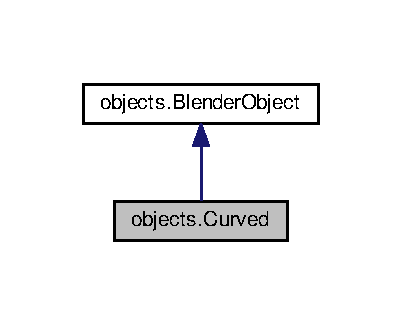
\includegraphics[width=193pt]{classobjects_1_1Curved__inherit__graph}
\end{center}
\end{figure}


Collaboration diagram for objects.\+Curved\+:\nopagebreak
\begin{figure}[H]
\begin{center}
\leavevmode
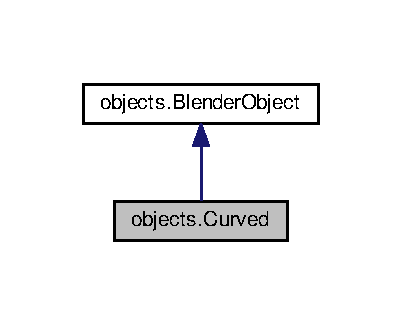
\includegraphics[width=193pt]{classobjects_1_1Curved__coll__graph}
\end{center}
\end{figure}
\subsection*{Public Member Functions}
\begin{DoxyCompactItemize}
\item 
def {\bfseries \+\_\+\+\_\+init\+\_\+\+\_\+} (self, p1, p2, p3, image=None)\hypertarget{classobjects_1_1Curved_a7236eb4a34e9120e88e8d8dde62cafef}{}\label{classobjects_1_1Curved_a7236eb4a34e9120e88e8d8dde62cafef}

\end{DoxyCompactItemize}
\subsection*{Public Attributes}
\begin{DoxyCompactItemize}
\item 
{\bfseries length}\hypertarget{classobjects_1_1Curved_a6c3e42fa031457afcfc292f3a4b34aa9}{}\label{classobjects_1_1Curved_a6c3e42fa031457afcfc292f3a4b34aa9}

\item 
{\bfseries radius}\hypertarget{classobjects_1_1Curved_ac9e8eb77597d2acd9d9aedaa3e59dcf2}{}\label{classobjects_1_1Curved_ac9e8eb77597d2acd9d9aedaa3e59dcf2}

\item 
{\bfseries n\+Faces}\hypertarget{classobjects_1_1Curved_ad47fa6e5dc6cc9cb3626c2bdf77cd0b6}{}\label{classobjects_1_1Curved_ad47fa6e5dc6cc9cb3626c2bdf77cd0b6}

\end{DoxyCompactItemize}
\subsection*{Static Public Attributes}
\begin{DoxyCompactItemize}
\item 
int {\bfseries n\+Faces} = 100\hypertarget{classobjects_1_1Curved_a1496f1fb48ba4463a606c21fc4c88e38}{}\label{classobjects_1_1Curved_a1496f1fb48ba4463a606c21fc4c88e38}

\item 
int {\bfseries radius} = 1\hypertarget{classobjects_1_1Curved_a91ca2bc31872df83d587f7cdd8b9bc95}{}\label{classobjects_1_1Curved_a91ca2bc31872df83d587f7cdd8b9bc95}

\item 
int {\bfseries length} = 5\hypertarget{classobjects_1_1Curved_a0590e97db4d2d7b1e44b1927030a5a3b}{}\label{classobjects_1_1Curved_a0590e97db4d2d7b1e44b1927030a5a3b}

\item 
list {\bfseries top\+\_\+face} = \mbox{[}$\,$\mbox{]}\hypertarget{classobjects_1_1Curved_aeff680dd5ec0b9a50d4df83bfd10ee7e}{}\label{classobjects_1_1Curved_aeff680dd5ec0b9a50d4df83bfd10ee7e}

\item 
list {\bfseries bot\+\_\+face} = \mbox{[}$\,$\mbox{]}\hypertarget{classobjects_1_1Curved_ae620bb9aa3c77c48b657fe82d0f93560}{}\label{classobjects_1_1Curved_ae620bb9aa3c77c48b657fe82d0f93560}

\item 
{\bfseries mesh} = None\hypertarget{classobjects_1_1Curved_aaa9b110af727e4fa82706cb45c8686fc}{}\label{classobjects_1_1Curved_aaa9b110af727e4fa82706cb45c8686fc}

\end{DoxyCompactItemize}


The documentation for this class was generated from the following file\+:\begin{DoxyCompactItemize}
\item 
/home/sebastian/catkin\+\_\+ws/src/animation\+\_\+render/scripts/framework/objects.\+py\end{DoxyCompactItemize}

\hypertarget{classobjects_1_1Cylinder}{}\section{objects.\+Cylinder Class Reference}
\label{classobjects_1_1Cylinder}\index{objects.\+Cylinder@{objects.\+Cylinder}}


Inheritance diagram for objects.\+Cylinder\+:\nopagebreak
\begin{figure}[H]
\begin{center}
\leavevmode
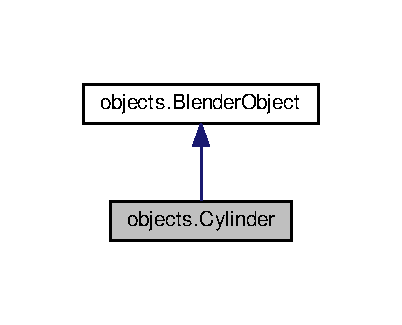
\includegraphics[width=193pt]{classobjects_1_1Cylinder__inherit__graph}
\end{center}
\end{figure}


Collaboration diagram for objects.\+Cylinder\+:\nopagebreak
\begin{figure}[H]
\begin{center}
\leavevmode
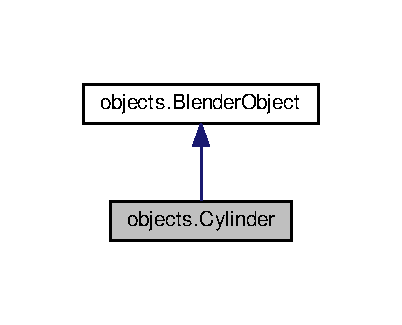
\includegraphics[width=193pt]{classobjects_1_1Cylinder__coll__graph}
\end{center}
\end{figure}
\subsection*{Public Member Functions}
\begin{DoxyCompactItemize}
\item 
def {\bfseries \+\_\+\+\_\+init\+\_\+\+\_\+} (self, p1, p2, p3, image=None)\hypertarget{classobjects_1_1Cylinder_acc80b3ae64195534aa7d1f8d49d50ced}{}\label{classobjects_1_1Cylinder_acc80b3ae64195534aa7d1f8d49d50ced}

\end{DoxyCompactItemize}
\subsection*{Public Attributes}
\begin{DoxyCompactItemize}
\item 
{\bfseries length}\hypertarget{classobjects_1_1Cylinder_a41d8b37a2c3543e62f36cda89aed7c7b}{}\label{classobjects_1_1Cylinder_a41d8b37a2c3543e62f36cda89aed7c7b}

\item 
{\bfseries radius}\hypertarget{classobjects_1_1Cylinder_a11f12e01ded26d6b315206e259b70b3e}{}\label{classobjects_1_1Cylinder_a11f12e01ded26d6b315206e259b70b3e}

\item 
{\bfseries n\+Faces}\hypertarget{classobjects_1_1Cylinder_a255a61ac30a16f8622004e3fac711c59}{}\label{classobjects_1_1Cylinder_a255a61ac30a16f8622004e3fac711c59}

\end{DoxyCompactItemize}
\subsection*{Static Public Attributes}
\begin{DoxyCompactItemize}
\item 
int {\bfseries n\+Faces} = 100\hypertarget{classobjects_1_1Cylinder_a557c65e8f5cc1a388e2e7e99454ab7b9}{}\label{classobjects_1_1Cylinder_a557c65e8f5cc1a388e2e7e99454ab7b9}

\item 
int {\bfseries radius} = 1\hypertarget{classobjects_1_1Cylinder_a240e394bea50a88b60390a0baa1d1062}{}\label{classobjects_1_1Cylinder_a240e394bea50a88b60390a0baa1d1062}

\item 
int {\bfseries length} = 5\hypertarget{classobjects_1_1Cylinder_ac4703036275d98d6add9747f3689fc17}{}\label{classobjects_1_1Cylinder_ac4703036275d98d6add9747f3689fc17}

\item 
list {\bfseries top\+\_\+face} = \mbox{[}$\,$\mbox{]}\hypertarget{classobjects_1_1Cylinder_a3d36e2847048c6414984b6ab35a0b777}{}\label{classobjects_1_1Cylinder_a3d36e2847048c6414984b6ab35a0b777}

\item 
list {\bfseries bot\+\_\+face} = \mbox{[}$\,$\mbox{]}\hypertarget{classobjects_1_1Cylinder_a816da9fabfa447e7df239a52aa2e78dc}{}\label{classobjects_1_1Cylinder_a816da9fabfa447e7df239a52aa2e78dc}

\item 
{\bfseries mesh} = None\hypertarget{classobjects_1_1Cylinder_a4ab88c3327bb56bddd2a086589247eb9}{}\label{classobjects_1_1Cylinder_a4ab88c3327bb56bddd2a086589247eb9}

\end{DoxyCompactItemize}


The documentation for this class was generated from the following file\+:\begin{DoxyCompactItemize}
\item 
/home/sebastian/catkin\+\_\+ws/src/animation\+\_\+render/scripts/framework/objects.\+py\end{DoxyCompactItemize}

\hypertarget{classanimations_1_1Example}{}\section{animations.\+Example Class Reference}
\label{classanimations_1_1Example}\index{animations.\+Example@{animations.\+Example}}


Inheritance diagram for animations.\+Example\+:\nopagebreak
\begin{figure}[H]
\begin{center}
\leavevmode
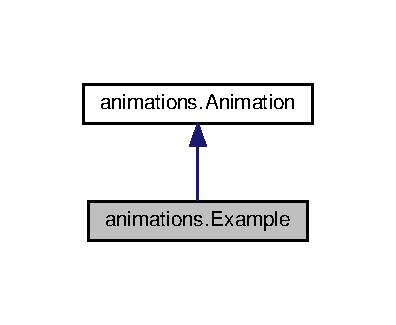
\includegraphics[width=190pt]{classanimations_1_1Example__inherit__graph}
\end{center}
\end{figure}


Collaboration diagram for animations.\+Example\+:\nopagebreak
\begin{figure}[H]
\begin{center}
\leavevmode
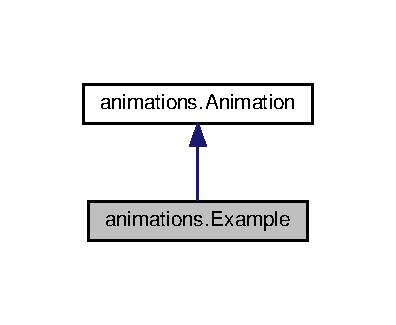
\includegraphics[width=190pt]{classanimations_1_1Example__coll__graph}
\end{center}
\end{figure}
\subsection*{Public Member Functions}
\begin{DoxyCompactItemize}
\item 
def {\bfseries \+\_\+\+\_\+init\+\_\+\+\_\+} (self, bdr\+\_\+handler, blender\+\_\+object, frames)\hypertarget{classanimations_1_1Example_ace7bc4cd0298fadf147fc372ca255b43}{}\label{classanimations_1_1Example_ace7bc4cd0298fadf147fc372ca255b43}

\end{DoxyCompactItemize}
\subsection*{Static Public Member Functions}
\begin{DoxyCompactItemize}
\item 
def {\bfseries get\+\_\+start\+\_\+position} ()\hypertarget{classanimations_1_1Example_a8eddeda3c2f74917e7be30890fd926da}{}\label{classanimations_1_1Example_a8eddeda3c2f74917e7be30890fd926da}

\item 
def {\bfseries get\+\_\+start\+\_\+rotation} ()\hypertarget{classanimations_1_1Example_a8788b5bf2835433ff6d3ec500724874d}{}\label{classanimations_1_1Example_a8788b5bf2835433ff6d3ec500724874d}

\end{DoxyCompactItemize}
\subsection*{Static Public Attributes}
\begin{DoxyCompactItemize}
\item 
string {\bfseries interpolation} = \textquotesingle{}L\+I\+N\+E\+AR\textquotesingle{}\hypertarget{classanimations_1_1Example_a80e3a095c082aea99b84b1e9cb7a2379}{}\label{classanimations_1_1Example_a80e3a095c082aea99b84b1e9cb7a2379}

\end{DoxyCompactItemize}


The documentation for this class was generated from the following file\+:\begin{DoxyCompactItemize}
\item 
/home/sebastian/catkin\+\_\+ws/src/animation\+\_\+render/scripts/framework/animations.\+py\end{DoxyCompactItemize}

\hypertarget{classanimations_1_1ForRender}{}\section{animations.\+For\+Render Class Reference}
\label{classanimations_1_1ForRender}\index{animations.\+For\+Render@{animations.\+For\+Render}}


Inheritance diagram for animations.\+For\+Render\+:\nopagebreak
\begin{figure}[H]
\begin{center}
\leavevmode
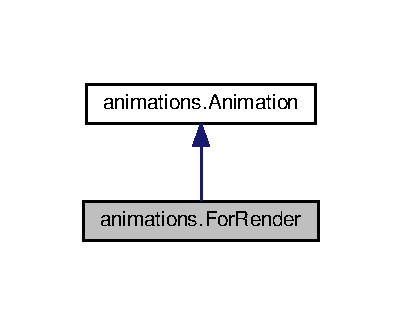
\includegraphics[width=193pt]{classanimations_1_1ForRender__inherit__graph}
\end{center}
\end{figure}


Collaboration diagram for animations.\+For\+Render\+:\nopagebreak
\begin{figure}[H]
\begin{center}
\leavevmode
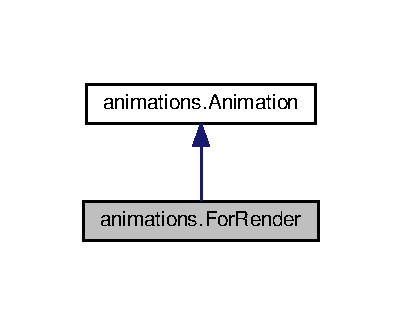
\includegraphics[width=193pt]{classanimations_1_1ForRender__coll__graph}
\end{center}
\end{figure}
\subsection*{Public Member Functions}
\begin{DoxyCompactItemize}
\item 
def {\bfseries \+\_\+\+\_\+init\+\_\+\+\_\+} (self, bdr\+\_\+handler, blender\+\_\+object, frames)\hypertarget{classanimations_1_1ForRender_a1ee4fa46efecc947a96953f5ff0d99b6}{}\label{classanimations_1_1ForRender_a1ee4fa46efecc947a96953f5ff0d99b6}

\end{DoxyCompactItemize}
\subsection*{Static Public Member Functions}
\begin{DoxyCompactItemize}
\item 
def {\bfseries get\+\_\+start\+\_\+position} ()\hypertarget{classanimations_1_1ForRender_a28d3cccf41dee0e9416d3630c7b6fdad}{}\label{classanimations_1_1ForRender_a28d3cccf41dee0e9416d3630c7b6fdad}

\item 
def {\bfseries get\+\_\+start\+\_\+rotation} ()\hypertarget{classanimations_1_1ForRender_a2cc55aedd12e789ca92c76f82cf314e3}{}\label{classanimations_1_1ForRender_a2cc55aedd12e789ca92c76f82cf314e3}

\end{DoxyCompactItemize}
\subsection*{Additional Inherited Members}


The documentation for this class was generated from the following file\+:\begin{DoxyCompactItemize}
\item 
/home/sebastian/catkin\+\_\+ws/src/animation\+\_\+render/scripts/framework/animations.\+py\end{DoxyCompactItemize}

\hypertarget{classanimations_1_1Movement2}{}\section{animations.\+Movement2 Class Reference}
\label{classanimations_1_1Movement2}\index{animations.\+Movement2@{animations.\+Movement2}}


Inheritance diagram for animations.\+Movement2\+:\nopagebreak
\begin{figure}[H]
\begin{center}
\leavevmode
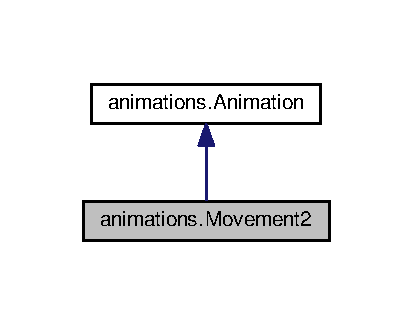
\includegraphics[width=198pt]{classanimations_1_1Movement2__inherit__graph}
\end{center}
\end{figure}


Collaboration diagram for animations.\+Movement2\+:\nopagebreak
\begin{figure}[H]
\begin{center}
\leavevmode
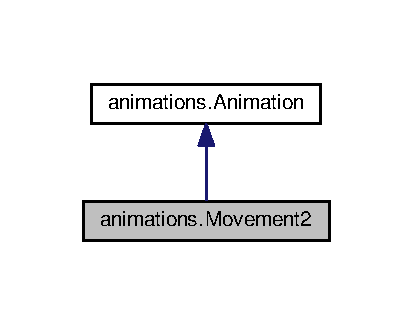
\includegraphics[width=198pt]{classanimations_1_1Movement2__coll__graph}
\end{center}
\end{figure}
\subsection*{Public Member Functions}
\begin{DoxyCompactItemize}
\item 
def {\bfseries \+\_\+\+\_\+init\+\_\+\+\_\+} (self, bdr\+\_\+handler, blender\+\_\+object, frames)\hypertarget{classanimations_1_1Movement2_a7f5da6078530b3041d7bd947a111a2f7}{}\label{classanimations_1_1Movement2_a7f5da6078530b3041d7bd947a111a2f7}

\end{DoxyCompactItemize}
\subsection*{Static Public Member Functions}
\begin{DoxyCompactItemize}
\item 
def {\bfseries get\+\_\+start\+\_\+position} ()\hypertarget{classanimations_1_1Movement2_ae6c38784e0dcc8de5acc4436f8b00194}{}\label{classanimations_1_1Movement2_ae6c38784e0dcc8de5acc4436f8b00194}

\item 
def {\bfseries get\+\_\+start\+\_\+rotation} ()\hypertarget{classanimations_1_1Movement2_a7be75ff5ba470a02fa3dbb136f60450e}{}\label{classanimations_1_1Movement2_a7be75ff5ba470a02fa3dbb136f60450e}

\end{DoxyCompactItemize}
\subsection*{Static Public Attributes}
\begin{DoxyCompactItemize}
\item 
string {\bfseries interpolation} = \textquotesingle{}L\+I\+N\+E\+AR\textquotesingle{}\hypertarget{classanimations_1_1Movement2_a7d01a8b034eb33518019e125a9bce03d}{}\label{classanimations_1_1Movement2_a7d01a8b034eb33518019e125a9bce03d}

\end{DoxyCompactItemize}


The documentation for this class was generated from the following file\+:\begin{DoxyCompactItemize}
\item 
/home/sebastian/catkin\+\_\+ws/src/animation\+\_\+render/scripts/framework/animations.\+py\end{DoxyCompactItemize}

\hypertarget{classanimations_1_1Movement3}{}\section{animations.\+Movement3 Class Reference}
\label{classanimations_1_1Movement3}\index{animations.\+Movement3@{animations.\+Movement3}}


Inheritance diagram for animations.\+Movement3\+:\nopagebreak
\begin{figure}[H]
\begin{center}
\leavevmode
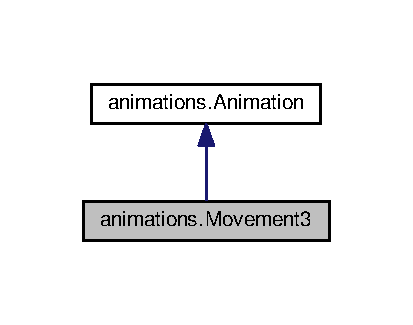
\includegraphics[width=198pt]{classanimations_1_1Movement3__inherit__graph}
\end{center}
\end{figure}


Collaboration diagram for animations.\+Movement3\+:\nopagebreak
\begin{figure}[H]
\begin{center}
\leavevmode
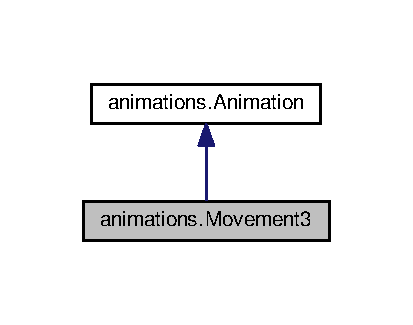
\includegraphics[width=198pt]{classanimations_1_1Movement3__coll__graph}
\end{center}
\end{figure}
\subsection*{Public Member Functions}
\begin{DoxyCompactItemize}
\item 
def {\bfseries \+\_\+\+\_\+init\+\_\+\+\_\+} (self, bdr\+\_\+handler, blender\+\_\+object, frames)\hypertarget{classanimations_1_1Movement3_a80d694eca808563a7b645a7230d8819a}{}\label{classanimations_1_1Movement3_a80d694eca808563a7b645a7230d8819a}

\end{DoxyCompactItemize}
\subsection*{Static Public Member Functions}
\begin{DoxyCompactItemize}
\item 
def {\bfseries get\+\_\+start\+\_\+position} ()\hypertarget{classanimations_1_1Movement3_a60a005812a73d0e6cd84a5f2597f9a4d}{}\label{classanimations_1_1Movement3_a60a005812a73d0e6cd84a5f2597f9a4d}

\item 
def {\bfseries get\+\_\+start\+\_\+rotation} ()\hypertarget{classanimations_1_1Movement3_acd418e86e75493b96bd0f701f9ef1979}{}\label{classanimations_1_1Movement3_acd418e86e75493b96bd0f701f9ef1979}

\end{DoxyCompactItemize}
\subsection*{Static Public Attributes}
\begin{DoxyCompactItemize}
\item 
string {\bfseries interpolation} = \textquotesingle{}L\+I\+N\+E\+AR\textquotesingle{}\hypertarget{classanimations_1_1Movement3_ad7792e03305d84e803c9b06bccbd65f1}{}\label{classanimations_1_1Movement3_ad7792e03305d84e803c9b06bccbd65f1}

\end{DoxyCompactItemize}


The documentation for this class was generated from the following file\+:\begin{DoxyCompactItemize}
\item 
/home/sebastian/catkin\+\_\+ws/src/animation\+\_\+render/scripts/framework/animations.\+py\end{DoxyCompactItemize}

\hypertarget{classanimations_1_1Movement4}{}\section{animations.\+Movement4 Class Reference}
\label{classanimations_1_1Movement4}\index{animations.\+Movement4@{animations.\+Movement4}}


Inheritance diagram for animations.\+Movement4\+:\nopagebreak
\begin{figure}[H]
\begin{center}
\leavevmode
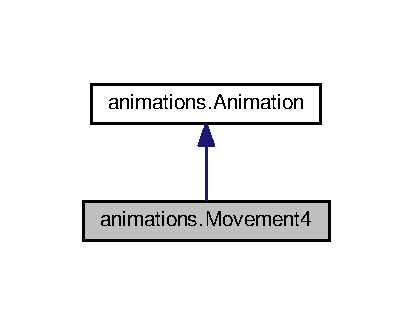
\includegraphics[width=198pt]{classanimations_1_1Movement4__inherit__graph}
\end{center}
\end{figure}


Collaboration diagram for animations.\+Movement4\+:\nopagebreak
\begin{figure}[H]
\begin{center}
\leavevmode
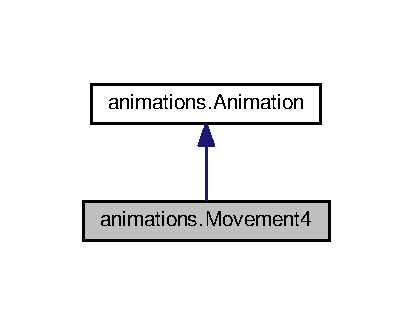
\includegraphics[width=198pt]{classanimations_1_1Movement4__coll__graph}
\end{center}
\end{figure}
\subsection*{Public Member Functions}
\begin{DoxyCompactItemize}
\item 
def {\bfseries \+\_\+\+\_\+init\+\_\+\+\_\+} (self, bdr\+\_\+handler, blender\+\_\+object, frames)\hypertarget{classanimations_1_1Movement4_a8bb1d458f8c33de7ea0f8b752df78115}{}\label{classanimations_1_1Movement4_a8bb1d458f8c33de7ea0f8b752df78115}

\end{DoxyCompactItemize}
\subsection*{Static Public Member Functions}
\begin{DoxyCompactItemize}
\item 
def {\bfseries get\+\_\+start\+\_\+position} ()\hypertarget{classanimations_1_1Movement4_a15c0a920408ffc6cf3ce5f0b3188ab8b}{}\label{classanimations_1_1Movement4_a15c0a920408ffc6cf3ce5f0b3188ab8b}

\item 
def {\bfseries get\+\_\+start\+\_\+rotation} ()\hypertarget{classanimations_1_1Movement4_a9733873769dc72c16cc20f847572e982}{}\label{classanimations_1_1Movement4_a9733873769dc72c16cc20f847572e982}

\end{DoxyCompactItemize}
\subsection*{Static Public Attributes}
\begin{DoxyCompactItemize}
\item 
string {\bfseries interpolation} = \textquotesingle{}L\+I\+N\+E\+AR\textquotesingle{}\hypertarget{classanimations_1_1Movement4_ae467b8a0ad3362dda80f9f5060e83d62}{}\label{classanimations_1_1Movement4_ae467b8a0ad3362dda80f9f5060e83d62}

\end{DoxyCompactItemize}


The documentation for this class was generated from the following file\+:\begin{DoxyCompactItemize}
\item 
/home/sebastian/catkin\+\_\+ws/src/animation\+\_\+render/scripts/framework/animations.\+py\end{DoxyCompactItemize}

\hypertarget{classobjects_1_1Plane}{}\section{objects.\+Plane Class Reference}
\label{classobjects_1_1Plane}\index{objects.\+Plane@{objects.\+Plane}}


Inheritance diagram for objects.\+Plane\+:\nopagebreak
\begin{figure}[H]
\begin{center}
\leavevmode
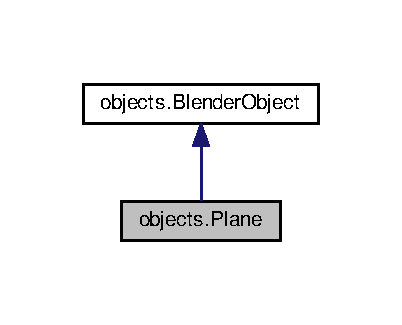
\includegraphics[width=193pt]{classobjects_1_1Plane__inherit__graph}
\end{center}
\end{figure}


Collaboration diagram for objects.\+Plane\+:\nopagebreak
\begin{figure}[H]
\begin{center}
\leavevmode
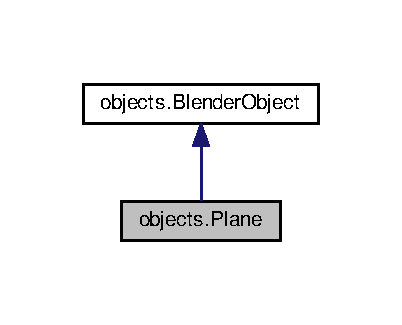
\includegraphics[width=193pt]{classobjects_1_1Plane__coll__graph}
\end{center}
\end{figure}
\subsection*{Public Member Functions}
\begin{DoxyCompactItemize}
\item 
def {\bfseries \+\_\+\+\_\+init\+\_\+\+\_\+} (self, p1, p2, p3, image=None)\hypertarget{classobjects_1_1Plane_ae5f23748ecc242d85aaa78f64d90bf38}{}\label{classobjects_1_1Plane_ae5f23748ecc242d85aaa78f64d90bf38}

\end{DoxyCompactItemize}
\subsection*{Static Public Attributes}
\begin{DoxyCompactItemize}
\item 
{\bfseries width} = None\hypertarget{classobjects_1_1Plane_adceffe68e570c2e4408ac5cde081291b}{}\label{classobjects_1_1Plane_adceffe68e570c2e4408ac5cde081291b}

\item 
{\bfseries height} = None\hypertarget{classobjects_1_1Plane_a47e939fe066057224263d2e8530f9438}{}\label{classobjects_1_1Plane_a47e939fe066057224263d2e8530f9438}

\end{DoxyCompactItemize}


The documentation for this class was generated from the following file\+:\begin{DoxyCompactItemize}
\item 
/home/sebastian/catkin\+\_\+ws/src/animation\+\_\+render/scripts/framework/objects.\+py\end{DoxyCompactItemize}

\hypertarget{structPose}{}\section{Pose Struct Reference}
\label{structPose}\index{Pose@{Pose}}
\subsection*{Public Attributes}
\begin{DoxyCompactItemize}
\item 
double {\bfseries x}\hypertarget{structPose_a0061c7789df90f593ab95118cbef387f}{}\label{structPose_a0061c7789df90f593ab95118cbef387f}

\item 
double {\bfseries y}\hypertarget{structPose_a6280216efe0840a7a55f025ad04e3b3d}{}\label{structPose_a6280216efe0840a7a55f025ad04e3b3d}

\item 
double {\bfseries z}\hypertarget{structPose_ad92c1d2873955b2bed6b29ac984858c3}{}\label{structPose_ad92c1d2873955b2bed6b29ac984858c3}

\item 
double {\bfseries ax}\hypertarget{structPose_a1ea6c02833ae2ecdca4d11e9379138e6}{}\label{structPose_a1ea6c02833ae2ecdca4d11e9379138e6}

\item 
double {\bfseries ay}\hypertarget{structPose_a6e7e21014c615126b38e08657d350063}{}\label{structPose_a6e7e21014c615126b38e08657d350063}

\item 
double {\bfseries az}\hypertarget{structPose_a0ae7c9f223b181c09da2f07cae7842c3}{}\label{structPose_a0ae7c9f223b181c09da2f07cae7842c3}

\end{DoxyCompactItemize}


The documentation for this struct was generated from the following file\+:\begin{DoxyCompactItemize}
\item 
/home/sebastian/catkin\+\_\+ws/src/animation\+\_\+render/src/pythoncaller.\+h\end{DoxyCompactItemize}

\hypertarget{classPythonCaller}{}\section{Python\+Caller Class Reference}
\label{classPythonCaller}\index{Python\+Caller@{Python\+Caller}}
\subsection*{Public Member Functions}
\begin{DoxyCompactItemize}
\item 
{\bfseries Python\+Caller} (ros\+::\+Node\+Handle $\ast$nh)\hypertarget{classPythonCaller_a17b5967b8cb382fa420dee33870a186a}{}\label{classPythonCaller_a17b5967b8cb382fa420dee33870a186a}

\item 
void \hyperlink{classPythonCaller_a2f996721a3cddabbfb9181d826fc9335}{render\+Video} (std\+::string video\+\_\+name, std\+::string template\+\_\+name, std\+::string background\+\_\+name, \hyperlink{structVideoOptions}{Video\+Options} video\+\_\+options, std\+::string object, std\+::string animation, double mp1, double mp2, double mp3)
\begin{DoxyCompactList}\small\item\em Render video. \end{DoxyCompactList}\item 
void \hyperlink{classPythonCaller_a2edcddb9119570ee95b2f4fb6e18c58c}{get\+Image\+List} (std\+::string path, int length, int min\+\_\+height, int min\+\_\+width, std\+::string keywords)
\begin{DoxyCompactList}\small\item\em Creates a list of image urls. \end{DoxyCompactList}\item 
void \hyperlink{classPythonCaller_a6217d7fc3432b3464c274b3fe2c5c539}{download\+Image} (std\+::string filename, std\+::string list, int nr)
\begin{DoxyCompactList}\small\item\em Download image from list. \end{DoxyCompactList}\item 
void \hyperlink{classPythonCaller_a4a7706b979cfe9aa45f1dcbc80d9a942}{get\+Ground\+Truth\+Data} (std\+::string animation, int frames, std\+::string path)
\begin{DoxyCompactList}\small\item\em Get the ground truth data of given animation. \end{DoxyCompactList}\item 
void \hyperlink{classPythonCaller_a690a2ad68abc1dc354eb74b9c58e65e7}{get\+Init\+Pose} (std\+::string animation, \hyperlink{structPose}{Pose} \&init\+Pose)
\begin{DoxyCompactList}\small\item\em Get init pose of animation. \end{DoxyCompactList}\end{DoxyCompactItemize}


\subsection{Member Function Documentation}
\index{Python\+Caller@{Python\+Caller}!download\+Image@{download\+Image}}
\index{download\+Image@{download\+Image}!Python\+Caller@{Python\+Caller}}
\subsubsection[{\texorpdfstring{download\+Image(std\+::string filename, std\+::string list, int nr)}{downloadImage(std::string filename, std::string list, int nr)}}]{\setlength{\rightskip}{0pt plus 5cm}void Python\+Caller\+::download\+Image (
\begin{DoxyParamCaption}
\item[{std\+::string}]{filename, }
\item[{std\+::string}]{list, }
\item[{int}]{nr}
\end{DoxyParamCaption}
)}\hypertarget{classPythonCaller_a6217d7fc3432b3464c274b3fe2c5c539}{}\label{classPythonCaller_a6217d7fc3432b3464c274b3fe2c5c539}


Download image from list. 


\begin{DoxyParams}{Parameters}
{\em nr} & Index of image \\
\hline
\end{DoxyParams}
\index{Python\+Caller@{Python\+Caller}!get\+Ground\+Truth\+Data@{get\+Ground\+Truth\+Data}}
\index{get\+Ground\+Truth\+Data@{get\+Ground\+Truth\+Data}!Python\+Caller@{Python\+Caller}}
\subsubsection[{\texorpdfstring{get\+Ground\+Truth\+Data(std\+::string animation, int frames, std\+::string path)}{getGroundTruthData(std::string animation, int frames, std::string path)}}]{\setlength{\rightskip}{0pt plus 5cm}void Python\+Caller\+::get\+Ground\+Truth\+Data (
\begin{DoxyParamCaption}
\item[{std\+::string}]{animation, }
\item[{int}]{frames, }
\item[{std\+::string}]{path}
\end{DoxyParamCaption}
)}\hypertarget{classPythonCaller_a4a7706b979cfe9aa45f1dcbc80d9a942}{}\label{classPythonCaller_a4a7706b979cfe9aa45f1dcbc80d9a942}


Get the ground truth data of given animation. 


\begin{DoxyParams}{Parameters}
{\em animation} & Name of animation \\
\hline
{\em frames} & Number of frames \\
\hline
{\em path} & output path \\
\hline
\end{DoxyParams}
\index{Python\+Caller@{Python\+Caller}!get\+Image\+List@{get\+Image\+List}}
\index{get\+Image\+List@{get\+Image\+List}!Python\+Caller@{Python\+Caller}}
\subsubsection[{\texorpdfstring{get\+Image\+List(std\+::string path, int length, int min\+\_\+height, int min\+\_\+width, std\+::string keywords)}{getImageList(std::string path, int length, int min_height, int min_width, std::string keywords)}}]{\setlength{\rightskip}{0pt plus 5cm}void Python\+Caller\+::get\+Image\+List (
\begin{DoxyParamCaption}
\item[{std\+::string}]{path, }
\item[{int}]{length, }
\item[{int}]{min\+\_\+height, }
\item[{int}]{min\+\_\+width, }
\item[{std\+::string}]{keywords}
\end{DoxyParamCaption}
)}\hypertarget{classPythonCaller_a2edcddb9119570ee95b2f4fb6e18c58c}{}\label{classPythonCaller_a2edcddb9119570ee95b2f4fb6e18c58c}


Creates a list of image urls. 


\begin{DoxyParams}{Parameters}
{\em length} & Length of list \\
\hline
{\em min\+\_\+height} & Minimal height of images \\
\hline
{\em min\+\_\+width} & Minimal width of images \\
\hline
{\em keywords} & Some keywords to search for \\
\hline
\end{DoxyParams}
\index{Python\+Caller@{Python\+Caller}!get\+Init\+Pose@{get\+Init\+Pose}}
\index{get\+Init\+Pose@{get\+Init\+Pose}!Python\+Caller@{Python\+Caller}}
\subsubsection[{\texorpdfstring{get\+Init\+Pose(std\+::string animation, Pose \&init\+Pose)}{getInitPose(std::string animation, Pose &initPose)}}]{\setlength{\rightskip}{0pt plus 5cm}void Python\+Caller\+::get\+Init\+Pose (
\begin{DoxyParamCaption}
\item[{std\+::string}]{animation, }
\item[{{\bf Pose} \&}]{init\+Pose}
\end{DoxyParamCaption}
)}\hypertarget{classPythonCaller_a690a2ad68abc1dc354eb74b9c58e65e7}{}\label{classPythonCaller_a690a2ad68abc1dc354eb74b9c58e65e7}


Get init pose of animation. 


\begin{DoxyParams}{Parameters}
{\em animation} & Name of animation \\
\hline
{\em x} & x position \\
\hline
{\em y} & y position \\
\hline
{\em z} & z position \\
\hline
{\em ax} & angle x \\
\hline
{\em ay} & angle y \\
\hline
{\em az} & angle z \\
\hline
\end{DoxyParams}
\index{Python\+Caller@{Python\+Caller}!render\+Video@{render\+Video}}
\index{render\+Video@{render\+Video}!Python\+Caller@{Python\+Caller}}
\subsubsection[{\texorpdfstring{render\+Video(std\+::string video\+\_\+name, std\+::string template\+\_\+name, std\+::string background\+\_\+name, Video\+Options video\+\_\+options, std\+::string object, std\+::string animation, double mp1, double mp2, double mp3)}{renderVideo(std::string video_name, std::string template_name, std::string background_name, VideoOptions video_options, std::string object, std::string animation, double mp1, double mp2, double mp3)}}]{\setlength{\rightskip}{0pt plus 5cm}void Python\+Caller\+::render\+Video (
\begin{DoxyParamCaption}
\item[{std\+::string}]{video\+\_\+name, }
\item[{std\+::string}]{template\+\_\+name, }
\item[{std\+::string}]{background\+\_\+name, }
\item[{{\bf Video\+Options}}]{video\+\_\+options, }
\item[{std\+::string}]{object, }
\item[{std\+::string}]{animation, }
\item[{double}]{mp1, }
\item[{double}]{mp2, }
\item[{double}]{mp3}
\end{DoxyParamCaption}
)}\hypertarget{classPythonCaller_a2f996721a3cddabbfb9181d826fc9335}{}\label{classPythonCaller_a2f996721a3cddabbfb9181d826fc9335}


Render video. 


\begin{DoxyParams}{Parameters}
{\em frames} & Number frames \\
\hline
{\em fps} & Frames per second \\
\hline
{\em object} & Name of object\+: Plane, Cylinder \\
\hline
{\em animation} & Name of animation \\
\hline
{\em res\+\_\+x} & Resolution x \\
\hline
{\em res\+\_\+y} & Resolution y \\
\hline
{\em mp1} & Model parameter 1 \\
\hline
{\em mp2} & Model parameter 2 \\
\hline
{\em mp3} & Model parameter 3 \\
\hline
\end{DoxyParams}


The documentation for this class was generated from the following files\+:\begin{DoxyCompactItemize}
\item 
/home/sebastian/catkin\+\_\+ws/src/animation\+\_\+render/src/pythoncaller.\+h\item 
/home/sebastian/catkin\+\_\+ws/src/animation\+\_\+render/src/pythoncaller.\+cpp\end{DoxyCompactItemize}

\hypertarget{classanimations_1_1RandomMixed}{}\section{animations.\+Random\+Mixed Class Reference}
\label{classanimations_1_1RandomMixed}\index{animations.\+Random\+Mixed@{animations.\+Random\+Mixed}}


Inheritance diagram for animations.\+Random\+Mixed\+:\nopagebreak
\begin{figure}[H]
\begin{center}
\leavevmode
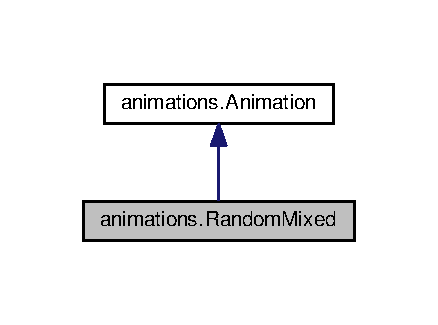
\includegraphics[width=210pt]{classanimations_1_1RandomMixed__inherit__graph}
\end{center}
\end{figure}


Collaboration diagram for animations.\+Random\+Mixed\+:\nopagebreak
\begin{figure}[H]
\begin{center}
\leavevmode
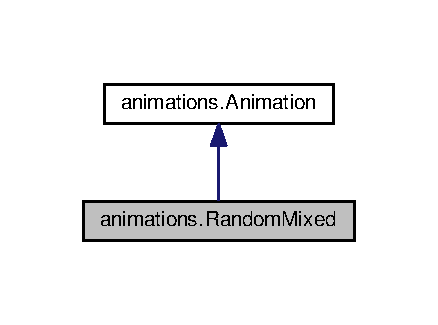
\includegraphics[width=210pt]{classanimations_1_1RandomMixed__coll__graph}
\end{center}
\end{figure}
\subsection*{Public Member Functions}
\begin{DoxyCompactItemize}
\item 
def {\bfseries \+\_\+\+\_\+init\+\_\+\+\_\+} (self, bdr\+\_\+handler, blender\+\_\+object, frames)\hypertarget{classanimations_1_1RandomMixed_ab68f35dacbe7599336810137f6d99eba}{}\label{classanimations_1_1RandomMixed_ab68f35dacbe7599336810137f6d99eba}

\end{DoxyCompactItemize}
\subsection*{Static Public Member Functions}
\begin{DoxyCompactItemize}
\item 
def {\bfseries get\+\_\+start\+\_\+position} ()\hypertarget{classanimations_1_1RandomMixed_a25fd7794d0df16789dce8df4004fb6b6}{}\label{classanimations_1_1RandomMixed_a25fd7794d0df16789dce8df4004fb6b6}

\item 
def {\bfseries get\+\_\+start\+\_\+rotation} ()\hypertarget{classanimations_1_1RandomMixed_a7a6872ce86fd30ae26b0f5c20a39dcc4}{}\label{classanimations_1_1RandomMixed_a7a6872ce86fd30ae26b0f5c20a39dcc4}

\end{DoxyCompactItemize}
\subsection*{Static Public Attributes}
\begin{DoxyCompactItemize}
\item 
string {\bfseries interpolation} = \textquotesingle{}L\+I\+N\+E\+AR\textquotesingle{}\hypertarget{classanimations_1_1RandomMixed_a7e47f9bfd4c90dccd8d5f9dfc64c119b}{}\label{classanimations_1_1RandomMixed_a7e47f9bfd4c90dccd8d5f9dfc64c119b}

\end{DoxyCompactItemize}


The documentation for this class was generated from the following file\+:\begin{DoxyCompactItemize}
\item 
/home/sebastian/catkin\+\_\+ws/src/animation\+\_\+render/scripts/framework/animations.\+py\end{DoxyCompactItemize}

\hypertarget{classanimations_1_1RandomMovement}{}\section{animations.\+Random\+Movement Class Reference}
\label{classanimations_1_1RandomMovement}\index{animations.\+Random\+Movement@{animations.\+Random\+Movement}}


Inheritance diagram for animations.\+Random\+Movement\+:\nopagebreak
\begin{figure}[H]
\begin{center}
\leavevmode
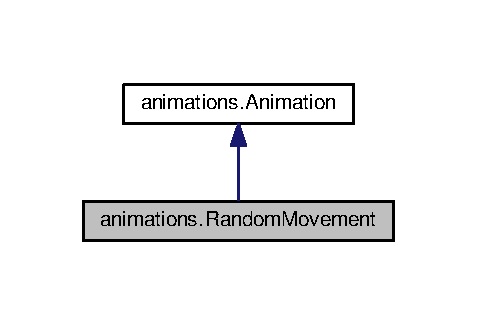
\includegraphics[width=229pt]{classanimations_1_1RandomMovement__inherit__graph}
\end{center}
\end{figure}


Collaboration diagram for animations.\+Random\+Movement\+:\nopagebreak
\begin{figure}[H]
\begin{center}
\leavevmode
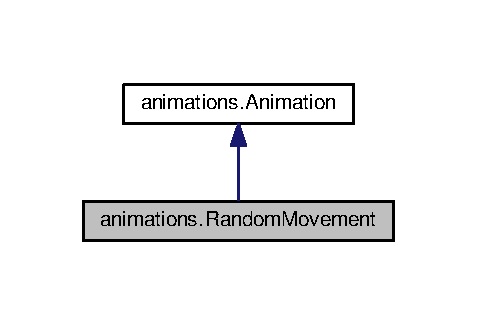
\includegraphics[width=229pt]{classanimations_1_1RandomMovement__coll__graph}
\end{center}
\end{figure}
\subsection*{Public Member Functions}
\begin{DoxyCompactItemize}
\item 
def {\bfseries \+\_\+\+\_\+init\+\_\+\+\_\+} (self, bdr\+\_\+handler, blender\+\_\+object, frames)\hypertarget{classanimations_1_1RandomMovement_ada9f89f50af67ffcd5c073a5e0672a20}{}\label{classanimations_1_1RandomMovement_ada9f89f50af67ffcd5c073a5e0672a20}

\end{DoxyCompactItemize}
\subsection*{Static Public Member Functions}
\begin{DoxyCompactItemize}
\item 
def {\bfseries get\+\_\+start\+\_\+position} ()\hypertarget{classanimations_1_1RandomMovement_a300ffa94c0c89728fc71adc65de61ed4}{}\label{classanimations_1_1RandomMovement_a300ffa94c0c89728fc71adc65de61ed4}

\item 
def {\bfseries get\+\_\+start\+\_\+rotation} ()\hypertarget{classanimations_1_1RandomMovement_aee4c35690406195b1e19ae0598d8420c}{}\label{classanimations_1_1RandomMovement_aee4c35690406195b1e19ae0598d8420c}

\end{DoxyCompactItemize}
\subsection*{Static Public Attributes}
\begin{DoxyCompactItemize}
\item 
string {\bfseries interpolation} = \textquotesingle{}L\+I\+N\+E\+AR\textquotesingle{}\hypertarget{classanimations_1_1RandomMovement_aba9ab6547454c34bdac3c29c00c1d0e7}{}\label{classanimations_1_1RandomMovement_aba9ab6547454c34bdac3c29c00c1d0e7}

\end{DoxyCompactItemize}


The documentation for this class was generated from the following file\+:\begin{DoxyCompactItemize}
\item 
/home/sebastian/catkin\+\_\+ws/src/animation\+\_\+render/scripts/framework/animations.\+py\end{DoxyCompactItemize}

\hypertarget{classanimations_1_1RandomRotation}{}\section{animations.\+Random\+Rotation Class Reference}
\label{classanimations_1_1RandomRotation}\index{animations.\+Random\+Rotation@{animations.\+Random\+Rotation}}


Inheritance diagram for animations.\+Random\+Rotation\+:\nopagebreak
\begin{figure}[H]
\begin{center}
\leavevmode
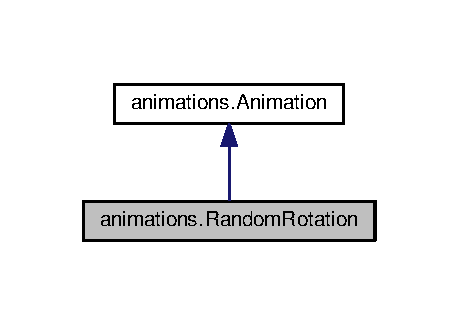
\includegraphics[width=220pt]{classanimations_1_1RandomRotation__inherit__graph}
\end{center}
\end{figure}


Collaboration diagram for animations.\+Random\+Rotation\+:\nopagebreak
\begin{figure}[H]
\begin{center}
\leavevmode
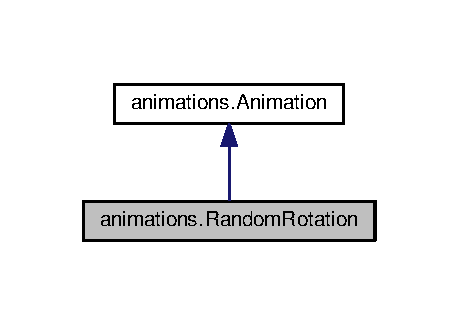
\includegraphics[width=220pt]{classanimations_1_1RandomRotation__coll__graph}
\end{center}
\end{figure}
\subsection*{Public Member Functions}
\begin{DoxyCompactItemize}
\item 
def {\bfseries \+\_\+\+\_\+init\+\_\+\+\_\+} (self, bdr\+\_\+handler, blender\+\_\+object, frames)\hypertarget{classanimations_1_1RandomRotation_ab61c1388a3fe39fd64de957e30ce14d7}{}\label{classanimations_1_1RandomRotation_ab61c1388a3fe39fd64de957e30ce14d7}

\end{DoxyCompactItemize}
\subsection*{Static Public Member Functions}
\begin{DoxyCompactItemize}
\item 
def {\bfseries get\+\_\+start\+\_\+position} ()\hypertarget{classanimations_1_1RandomRotation_a9115fe253a9309aa7b55add687460bf2}{}\label{classanimations_1_1RandomRotation_a9115fe253a9309aa7b55add687460bf2}

\item 
def {\bfseries get\+\_\+start\+\_\+rotation} ()\hypertarget{classanimations_1_1RandomRotation_a74c70c2aa40cec8cae4dd74a39befe8a}{}\label{classanimations_1_1RandomRotation_a74c70c2aa40cec8cae4dd74a39befe8a}

\end{DoxyCompactItemize}
\subsection*{Static Public Attributes}
\begin{DoxyCompactItemize}
\item 
string {\bfseries interpolation} = \textquotesingle{}L\+I\+N\+E\+AR\textquotesingle{}\hypertarget{classanimations_1_1RandomRotation_ab40853a968d7bcd7c32c0a7e67801340}{}\label{classanimations_1_1RandomRotation_ab40853a968d7bcd7c32c0a7e67801340}

\end{DoxyCompactItemize}


The documentation for this class was generated from the following file\+:\begin{DoxyCompactItemize}
\item 
/home/sebastian/catkin\+\_\+ws/src/animation\+\_\+render/scripts/framework/animations.\+py\end{DoxyCompactItemize}

\hypertarget{classanimations_1_1RenderTest}{}\section{animations.\+Render\+Test Class Reference}
\label{classanimations_1_1RenderTest}\index{animations.\+Render\+Test@{animations.\+Render\+Test}}


Inheritance diagram for animations.\+Render\+Test\+:\nopagebreak
\begin{figure}[H]
\begin{center}
\leavevmode
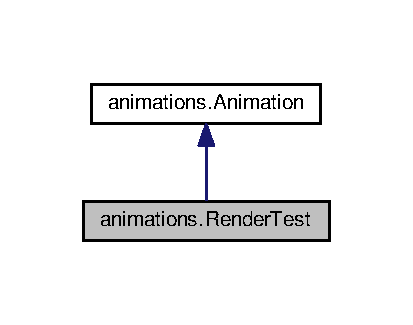
\includegraphics[width=198pt]{classanimations_1_1RenderTest__inherit__graph}
\end{center}
\end{figure}


Collaboration diagram for animations.\+Render\+Test\+:\nopagebreak
\begin{figure}[H]
\begin{center}
\leavevmode
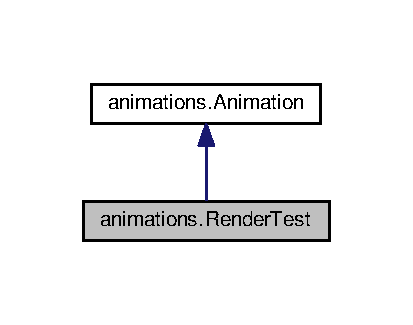
\includegraphics[width=198pt]{classanimations_1_1RenderTest__coll__graph}
\end{center}
\end{figure}
\subsection*{Public Member Functions}
\begin{DoxyCompactItemize}
\item 
def {\bfseries \+\_\+\+\_\+init\+\_\+\+\_\+} (self, bdr\+\_\+handler, blender\+\_\+object, frames)\hypertarget{classanimations_1_1RenderTest_a66f89be63f34c2ee2906c0039f2b1035}{}\label{classanimations_1_1RenderTest_a66f89be63f34c2ee2906c0039f2b1035}

\end{DoxyCompactItemize}
\subsection*{Static Public Member Functions}
\begin{DoxyCompactItemize}
\item 
def {\bfseries get\+\_\+start\+\_\+position} ()\hypertarget{classanimations_1_1RenderTest_ade0bab75701081a627ed090b19389277}{}\label{classanimations_1_1RenderTest_ade0bab75701081a627ed090b19389277}

\item 
def {\bfseries get\+\_\+start\+\_\+rotation} ()\hypertarget{classanimations_1_1RenderTest_a170b1a2bb03110dc77a76e6a845ccf27}{}\label{classanimations_1_1RenderTest_a170b1a2bb03110dc77a76e6a845ccf27}

\end{DoxyCompactItemize}
\subsection*{Additional Inherited Members}


The documentation for this class was generated from the following file\+:\begin{DoxyCompactItemize}
\item 
/home/sebastian/catkin\+\_\+ws/src/animation\+\_\+render/scripts/framework/animations.\+py\end{DoxyCompactItemize}

\hypertarget{classanimations_1_1RotationX}{}\section{animations.\+RotationX Class Reference}
\label{classanimations_1_1RotationX}\index{animations.\+RotationX@{animations.\+RotationX}}


Inheritance diagram for animations.\+RotationX\+:\nopagebreak
\begin{figure}[H]
\begin{center}
\leavevmode
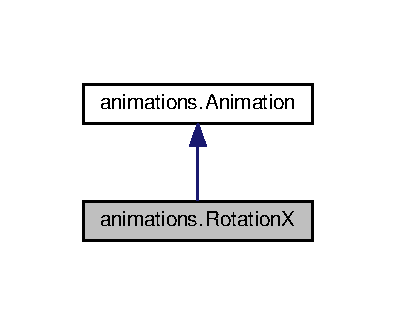
\includegraphics[width=190pt]{classanimations_1_1RotationX__inherit__graph}
\end{center}
\end{figure}


Collaboration diagram for animations.\+RotationX\+:\nopagebreak
\begin{figure}[H]
\begin{center}
\leavevmode
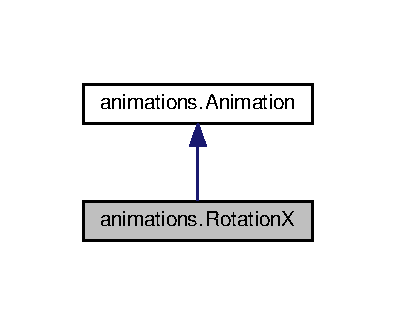
\includegraphics[width=190pt]{classanimations_1_1RotationX__coll__graph}
\end{center}
\end{figure}
\subsection*{Public Member Functions}
\begin{DoxyCompactItemize}
\item 
def {\bfseries \+\_\+\+\_\+init\+\_\+\+\_\+} (self, bdr\+\_\+handler, blender\+\_\+object, frames)\hypertarget{classanimations_1_1RotationX_af029701a0cd697e00673d505903dbf7d}{}\label{classanimations_1_1RotationX_af029701a0cd697e00673d505903dbf7d}

\end{DoxyCompactItemize}
\subsection*{Static Public Member Functions}
\begin{DoxyCompactItemize}
\item 
def {\bfseries get\+\_\+start\+\_\+position} ()\hypertarget{classanimations_1_1RotationX_a840627b45d0250a98f2e2444d11c83db}{}\label{classanimations_1_1RotationX_a840627b45d0250a98f2e2444d11c83db}

\item 
def {\bfseries get\+\_\+start\+\_\+rotation} ()\hypertarget{classanimations_1_1RotationX_a354b17e739f97e51d11ba01737986c97}{}\label{classanimations_1_1RotationX_a354b17e739f97e51d11ba01737986c97}

\end{DoxyCompactItemize}
\subsection*{Static Public Attributes}
\begin{DoxyCompactItemize}
\item 
string {\bfseries interpolation} = \textquotesingle{}Q\+U\+AD\textquotesingle{}\hypertarget{classanimations_1_1RotationX_a7527568a07d99d40d3e130d1810bda19}{}\label{classanimations_1_1RotationX_a7527568a07d99d40d3e130d1810bda19}

\end{DoxyCompactItemize}


The documentation for this class was generated from the following file\+:\begin{DoxyCompactItemize}
\item 
/home/sebastian/catkin\+\_\+ws/src/animation\+\_\+render/scripts/framework/animations.\+py\end{DoxyCompactItemize}

\hypertarget{classanimations_1_1RotationX2}{}\section{animations.\+Rotation\+X2 Class Reference}
\label{classanimations_1_1RotationX2}\index{animations.\+Rotation\+X2@{animations.\+Rotation\+X2}}


Inheritance diagram for animations.\+Rotation\+X2\+:\nopagebreak
\begin{figure}[H]
\begin{center}
\leavevmode
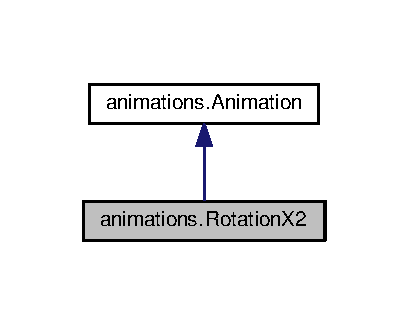
\includegraphics[width=196pt]{classanimations_1_1RotationX2__inherit__graph}
\end{center}
\end{figure}


Collaboration diagram for animations.\+Rotation\+X2\+:\nopagebreak
\begin{figure}[H]
\begin{center}
\leavevmode
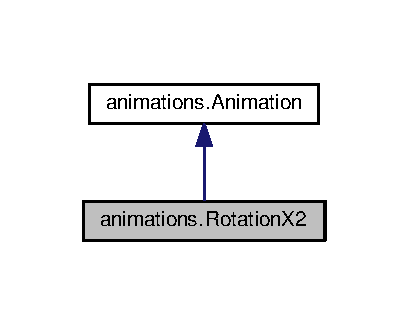
\includegraphics[width=196pt]{classanimations_1_1RotationX2__coll__graph}
\end{center}
\end{figure}
\subsection*{Public Member Functions}
\begin{DoxyCompactItemize}
\item 
def {\bfseries \+\_\+\+\_\+init\+\_\+\+\_\+} (self, bdr\+\_\+handler, blender\+\_\+object, frames)\hypertarget{classanimations_1_1RotationX2_ac9330a17bdf3ad662921c5f44bf77534}{}\label{classanimations_1_1RotationX2_ac9330a17bdf3ad662921c5f44bf77534}

\end{DoxyCompactItemize}
\subsection*{Static Public Member Functions}
\begin{DoxyCompactItemize}
\item 
def {\bfseries get\+\_\+start\+\_\+position} ()\hypertarget{classanimations_1_1RotationX2_a84666356519c5aa6cb8554adbfd38035}{}\label{classanimations_1_1RotationX2_a84666356519c5aa6cb8554adbfd38035}

\item 
def {\bfseries get\+\_\+start\+\_\+rotation} ()\hypertarget{classanimations_1_1RotationX2_aa47a12773110af6516bc79d1cf72128e}{}\label{classanimations_1_1RotationX2_aa47a12773110af6516bc79d1cf72128e}

\end{DoxyCompactItemize}
\subsection*{Static Public Attributes}
\begin{DoxyCompactItemize}
\item 
string {\bfseries interpolation} = \textquotesingle{}Q\+U\+AD\textquotesingle{}\hypertarget{classanimations_1_1RotationX2_a2e235ccda5d2db4442a0d60a80806797}{}\label{classanimations_1_1RotationX2_a2e235ccda5d2db4442a0d60a80806797}

\end{DoxyCompactItemize}


The documentation for this class was generated from the following file\+:\begin{DoxyCompactItemize}
\item 
/home/sebastian/catkin\+\_\+ws/src/animation\+\_\+render/scripts/framework/animations.\+py\end{DoxyCompactItemize}

\hypertarget{classanimations_1_1RotationXacc}{}\section{animations.\+Rotation\+Xacc Class Reference}
\label{classanimations_1_1RotationXacc}\index{animations.\+Rotation\+Xacc@{animations.\+Rotation\+Xacc}}


Inheritance diagram for animations.\+Rotation\+Xacc\+:\nopagebreak
\begin{figure}[H]
\begin{center}
\leavevmode
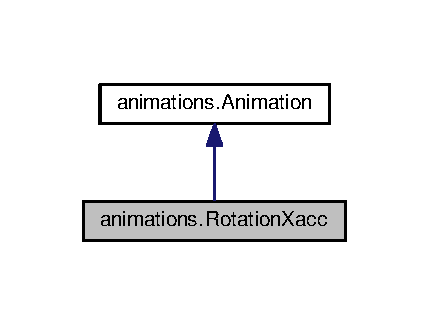
\includegraphics[width=206pt]{classanimations_1_1RotationXacc__inherit__graph}
\end{center}
\end{figure}


Collaboration diagram for animations.\+Rotation\+Xacc\+:\nopagebreak
\begin{figure}[H]
\begin{center}
\leavevmode
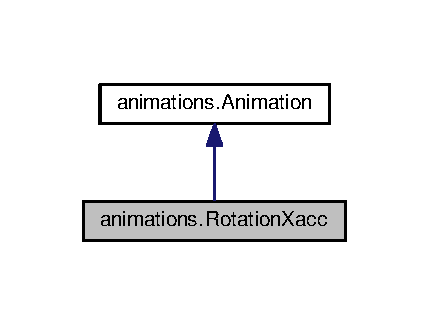
\includegraphics[width=206pt]{classanimations_1_1RotationXacc__coll__graph}
\end{center}
\end{figure}
\subsection*{Public Member Functions}
\begin{DoxyCompactItemize}
\item 
def {\bfseries \+\_\+\+\_\+init\+\_\+\+\_\+} (self, bdr\+\_\+handler, blender\+\_\+object, frames)\hypertarget{classanimations_1_1RotationXacc_a4caf5eee56e20df906754de30f9cc213}{}\label{classanimations_1_1RotationXacc_a4caf5eee56e20df906754de30f9cc213}

\end{DoxyCompactItemize}
\subsection*{Static Public Member Functions}
\begin{DoxyCompactItemize}
\item 
def {\bfseries get\+\_\+start\+\_\+position} ()\hypertarget{classanimations_1_1RotationXacc_a235dfb6d67464c06506ea16249e19492}{}\label{classanimations_1_1RotationXacc_a235dfb6d67464c06506ea16249e19492}

\item 
def {\bfseries get\+\_\+start\+\_\+rotation} ()\hypertarget{classanimations_1_1RotationXacc_ac1b325a7fc916327b955935177e3fa5f}{}\label{classanimations_1_1RotationXacc_ac1b325a7fc916327b955935177e3fa5f}

\end{DoxyCompactItemize}
\subsection*{Static Public Attributes}
\begin{DoxyCompactItemize}
\item 
string {\bfseries interpolation} = \textquotesingle{}Q\+U\+AD\textquotesingle{}\hypertarget{classanimations_1_1RotationXacc_a8396c8e72dd7cba7618b9e9f154d0209}{}\label{classanimations_1_1RotationXacc_a8396c8e72dd7cba7618b9e9f154d0209}

\end{DoxyCompactItemize}


The documentation for this class was generated from the following file\+:\begin{DoxyCompactItemize}
\item 
/home/sebastian/catkin\+\_\+ws/src/animation\+\_\+render/scripts/framework/animations.\+py\end{DoxyCompactItemize}

\hypertarget{classanimations_1_1RotationY}{}\section{animations.\+RotationY Class Reference}
\label{classanimations_1_1RotationY}\index{animations.\+RotationY@{animations.\+RotationY}}


Inheritance diagram for animations.\+RotationY\+:\nopagebreak
\begin{figure}[H]
\begin{center}
\leavevmode
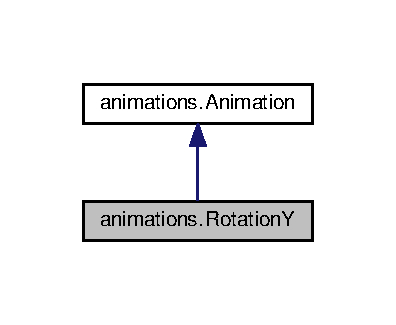
\includegraphics[width=190pt]{classanimations_1_1RotationY__inherit__graph}
\end{center}
\end{figure}


Collaboration diagram for animations.\+RotationY\+:\nopagebreak
\begin{figure}[H]
\begin{center}
\leavevmode
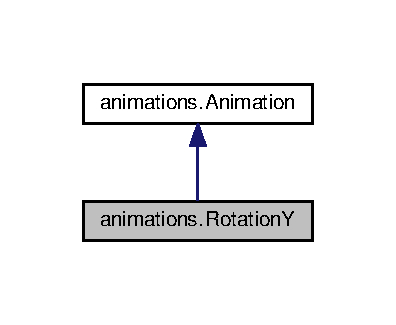
\includegraphics[width=190pt]{classanimations_1_1RotationY__coll__graph}
\end{center}
\end{figure}
\subsection*{Public Member Functions}
\begin{DoxyCompactItemize}
\item 
def {\bfseries \+\_\+\+\_\+init\+\_\+\+\_\+} (self, bdr\+\_\+handler, blender\+\_\+object, frames)\hypertarget{classanimations_1_1RotationY_ae56ace68b18a080aefbf96be9306e107}{}\label{classanimations_1_1RotationY_ae56ace68b18a080aefbf96be9306e107}

\end{DoxyCompactItemize}
\subsection*{Static Public Member Functions}
\begin{DoxyCompactItemize}
\item 
def {\bfseries get\+\_\+start\+\_\+position} ()\hypertarget{classanimations_1_1RotationY_a30f3604aec407b004e8abcc713c34dd6}{}\label{classanimations_1_1RotationY_a30f3604aec407b004e8abcc713c34dd6}

\item 
def {\bfseries get\+\_\+start\+\_\+rotation} ()\hypertarget{classanimations_1_1RotationY_abe2b559c413d71d183fd8259e4d02053}{}\label{classanimations_1_1RotationY_abe2b559c413d71d183fd8259e4d02053}

\end{DoxyCompactItemize}
\subsection*{Static Public Attributes}
\begin{DoxyCompactItemize}
\item 
string {\bfseries interpolation} = \textquotesingle{}L\+I\+N\+E\+AR\textquotesingle{}\hypertarget{classanimations_1_1RotationY_af2106c568132f7af7789b153fa1fccc7}{}\label{classanimations_1_1RotationY_af2106c568132f7af7789b153fa1fccc7}

\end{DoxyCompactItemize}


The documentation for this class was generated from the following file\+:\begin{DoxyCompactItemize}
\item 
/home/sebastian/catkin\+\_\+ws/src/animation\+\_\+render/scripts/framework/animations.\+py\end{DoxyCompactItemize}

\hypertarget{classanimations_1_1RotationZ}{}\section{animations.\+RotationZ Class Reference}
\label{classanimations_1_1RotationZ}\index{animations.\+RotationZ@{animations.\+RotationZ}}


Inheritance diagram for animations.\+RotationZ\+:\nopagebreak
\begin{figure}[H]
\begin{center}
\leavevmode
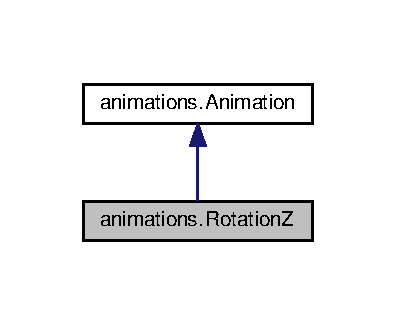
\includegraphics[width=190pt]{classanimations_1_1RotationZ__inherit__graph}
\end{center}
\end{figure}


Collaboration diagram for animations.\+RotationZ\+:\nopagebreak
\begin{figure}[H]
\begin{center}
\leavevmode
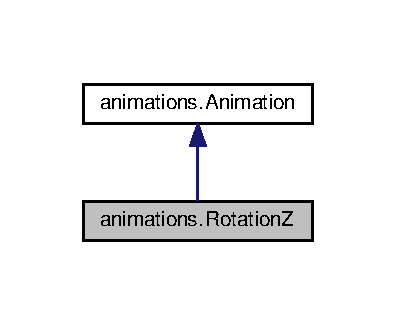
\includegraphics[width=190pt]{classanimations_1_1RotationZ__coll__graph}
\end{center}
\end{figure}
\subsection*{Public Member Functions}
\begin{DoxyCompactItemize}
\item 
def {\bfseries \+\_\+\+\_\+init\+\_\+\+\_\+} (self, bdr\+\_\+handler, blender\+\_\+object, frames)\hypertarget{classanimations_1_1RotationZ_a160c6953e9099be9ed0bd9cc565a15b3}{}\label{classanimations_1_1RotationZ_a160c6953e9099be9ed0bd9cc565a15b3}

\end{DoxyCompactItemize}
\subsection*{Static Public Member Functions}
\begin{DoxyCompactItemize}
\item 
def {\bfseries get\+\_\+start\+\_\+position} ()\hypertarget{classanimations_1_1RotationZ_a284c52c6b00f8f73b0ca80e4f15d07b8}{}\label{classanimations_1_1RotationZ_a284c52c6b00f8f73b0ca80e4f15d07b8}

\item 
def {\bfseries get\+\_\+start\+\_\+rotation} ()\hypertarget{classanimations_1_1RotationZ_a16fa2ead84238670e41d9025f7dd93f0}{}\label{classanimations_1_1RotationZ_a16fa2ead84238670e41d9025f7dd93f0}

\end{DoxyCompactItemize}
\subsection*{Static Public Attributes}
\begin{DoxyCompactItemize}
\item 
string {\bfseries interpolation} = \textquotesingle{}Q\+U\+AD\textquotesingle{}\hypertarget{classanimations_1_1RotationZ_aadf3b70e2c87073e84f3f153cdf1b37b}{}\label{classanimations_1_1RotationZ_aadf3b70e2c87073e84f3f153cdf1b37b}

\end{DoxyCompactItemize}


The documentation for this class was generated from the following file\+:\begin{DoxyCompactItemize}
\item 
/home/sebastian/catkin\+\_\+ws/src/animation\+\_\+render/scripts/framework/animations.\+py\end{DoxyCompactItemize}

\hypertarget{classTemplateEvaluation}{}\section{Template\+Evaluation Class Reference}
\label{classTemplateEvaluation}\index{Template\+Evaluation@{Template\+Evaluation}}
\subsection*{Public Member Functions}
\begin{DoxyCompactItemize}
\item 
{\bfseries Template\+Evaluation} (double t\+\_\+grad, double t\+\_\+acc)\hypertarget{classTemplateEvaluation_aae06cd355b4c4a03221527612ef85c1f}{}\label{classTemplateEvaluation_aae06cd355b4c4a03221527612ef85c1f}

\item 
bool {\bfseries evaluate} (std\+::string file)\hypertarget{classTemplateEvaluation_a95f928c675000aee3dbf079b7853eb7a}{}\label{classTemplateEvaluation_a95f928c675000aee3dbf079b7853eb7a}

\item 
bool {\bfseries evaluate} (std\+::string file, double \&acc\+\_\+x, double \&acc\+\_\+y)\hypertarget{classTemplateEvaluation_a3b086c476e5c526cfd171cc3b6d476d3}{}\label{classTemplateEvaluation_a3b086c476e5c526cfd171cc3b6d476d3}

\item 
bool {\bfseries evaluate2} (std\+::string file)\hypertarget{classTemplateEvaluation_a55fc26b317e77696133370fc12088be4}{}\label{classTemplateEvaluation_a55fc26b317e77696133370fc12088be4}

\item 
bool {\bfseries evaluate3} (std\+::string file, bool out=false)\hypertarget{classTemplateEvaluation_a0d195cb1639286f3b0c380af1b1e3da4}{}\label{classTemplateEvaluation_a0d195cb1639286f3b0c380af1b1e3da4}

\item 
bool {\bfseries evaluate4} (std\+::string file, bool out=false)\hypertarget{classTemplateEvaluation_a24e7297912bb5ee73b808e39227409b0}{}\label{classTemplateEvaluation_a24e7297912bb5ee73b808e39227409b0}

\item 
bool {\bfseries evaluate5} (std\+::string file, bool out=false)\hypertarget{classTemplateEvaluation_af23cc659648615f75baefc996b7e13d0}{}\label{classTemplateEvaluation_af23cc659648615f75baefc996b7e13d0}

\item 
void {\bfseries export\+Data} (std\+::string path, std\+::string file)\hypertarget{classTemplateEvaluation_ad7ac1c323d282e27103a00c25ac8dd85}{}\label{classTemplateEvaluation_ad7ac1c323d282e27103a00c25ac8dd85}

\end{DoxyCompactItemize}
\subsection*{Static Public Member Functions}
\begin{DoxyCompactItemize}
\item 
static bool {\bfseries show\+Image} (std\+::string path)\hypertarget{classTemplateEvaluation_acae88596fe4a036aaef38d204ab0490c}{}\label{classTemplateEvaluation_acae88596fe4a036aaef38d204ab0490c}

\end{DoxyCompactItemize}
\subsection*{Public Attributes}
\begin{DoxyCompactItemize}
\item 
double {\bfseries m\+Grad\+Threshold}\hypertarget{classTemplateEvaluation_a4cab1aa578ca994414f7885f6289c77e}{}\label{classTemplateEvaluation_a4cab1aa578ca994414f7885f6289c77e}

\item 
double {\bfseries m\+Acceptance\+Threshold}\hypertarget{classTemplateEvaluation_aacc5ef9db56038a2ed5a001451c0e36b}{}\label{classTemplateEvaluation_aacc5ef9db56038a2ed5a001451c0e36b}

\end{DoxyCompactItemize}


The documentation for this class was generated from the following files\+:\begin{DoxyCompactItemize}
\item 
/home/sebastian/catkin\+\_\+ws/src/animation\+\_\+render/src/templateevaluation.\+h\item 
/home/sebastian/catkin\+\_\+ws/src/animation\+\_\+render/src/templateevaluation.\+cpp\end{DoxyCompactItemize}

\hypertarget{classanimations_1_1TranslationX}{}\section{animations.\+TranslationX Class Reference}
\label{classanimations_1_1TranslationX}\index{animations.\+TranslationX@{animations.\+TranslationX}}


Inheritance diagram for animations.\+TranslationX\+:\nopagebreak
\begin{figure}[H]
\begin{center}
\leavevmode
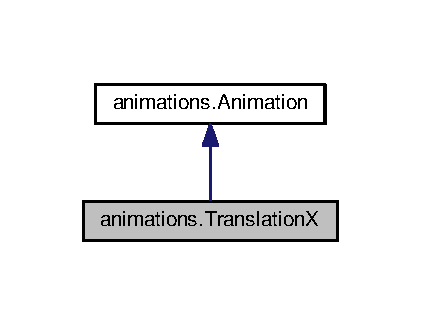
\includegraphics[width=202pt]{classanimations_1_1TranslationX__inherit__graph}
\end{center}
\end{figure}


Collaboration diagram for animations.\+TranslationX\+:\nopagebreak
\begin{figure}[H]
\begin{center}
\leavevmode
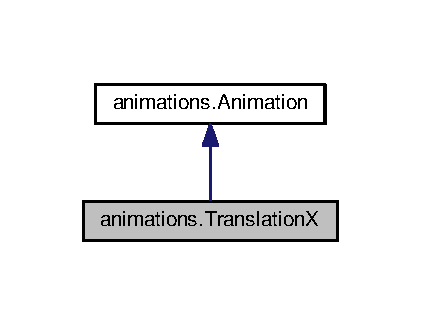
\includegraphics[width=202pt]{classanimations_1_1TranslationX__coll__graph}
\end{center}
\end{figure}
\subsection*{Public Member Functions}
\begin{DoxyCompactItemize}
\item 
def {\bfseries \+\_\+\+\_\+init\+\_\+\+\_\+} (self, bdr\+\_\+handler, blender\+\_\+object, frames)\hypertarget{classanimations_1_1TranslationX_af68a0c8030c1d67f71ab91967900d3d2}{}\label{classanimations_1_1TranslationX_af68a0c8030c1d67f71ab91967900d3d2}

\end{DoxyCompactItemize}
\subsection*{Static Public Member Functions}
\begin{DoxyCompactItemize}
\item 
def {\bfseries get\+\_\+start\+\_\+rotation} ()\hypertarget{classanimations_1_1TranslationX_a6df21799e865f0150db671b978d227a6}{}\label{classanimations_1_1TranslationX_a6df21799e865f0150db671b978d227a6}

\item 
def {\bfseries get\+\_\+start\+\_\+position} ()\hypertarget{classanimations_1_1TranslationX_a7f2871abe9c9ac4eceab0a412074ff7c}{}\label{classanimations_1_1TranslationX_a7f2871abe9c9ac4eceab0a412074ff7c}

\end{DoxyCompactItemize}
\subsection*{Static Public Attributes}
\begin{DoxyCompactItemize}
\item 
string {\bfseries interpolation} = \textquotesingle{}L\+I\+N\+E\+AR\textquotesingle{}\hypertarget{classanimations_1_1TranslationX_ad1729c2600ad2816247ab67842da7361}{}\label{classanimations_1_1TranslationX_ad1729c2600ad2816247ab67842da7361}

\end{DoxyCompactItemize}


The documentation for this class was generated from the following file\+:\begin{DoxyCompactItemize}
\item 
/home/sebastian/catkin\+\_\+ws/src/animation\+\_\+render/scripts/framework/animations.\+py\end{DoxyCompactItemize}

\hypertarget{classanimations_1_1TranslationX2}{}\section{animations.\+Translation\+X2 Class Reference}
\label{classanimations_1_1TranslationX2}\index{animations.\+Translation\+X2@{animations.\+Translation\+X2}}


Inheritance diagram for animations.\+Translation\+X2\+:\nopagebreak
\begin{figure}[H]
\begin{center}
\leavevmode
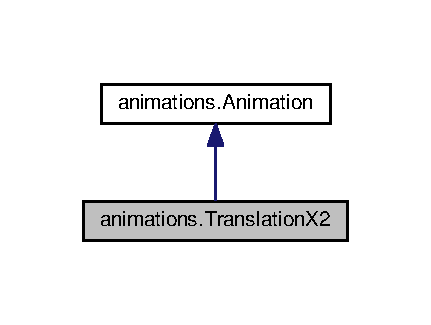
\includegraphics[width=207pt]{classanimations_1_1TranslationX2__inherit__graph}
\end{center}
\end{figure}


Collaboration diagram for animations.\+Translation\+X2\+:\nopagebreak
\begin{figure}[H]
\begin{center}
\leavevmode
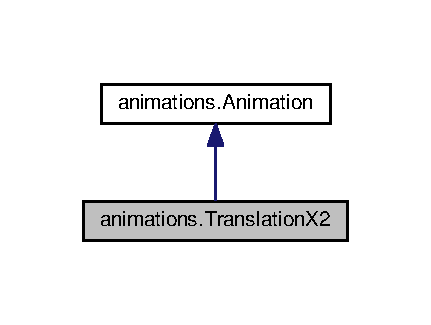
\includegraphics[width=207pt]{classanimations_1_1TranslationX2__coll__graph}
\end{center}
\end{figure}
\subsection*{Public Member Functions}
\begin{DoxyCompactItemize}
\item 
def {\bfseries \+\_\+\+\_\+init\+\_\+\+\_\+} (self, bdr\+\_\+handler, blender\+\_\+object, frames)\hypertarget{classanimations_1_1TranslationX2_a737b82d641d35f73a5072242097aba2e}{}\label{classanimations_1_1TranslationX2_a737b82d641d35f73a5072242097aba2e}

\end{DoxyCompactItemize}
\subsection*{Static Public Member Functions}
\begin{DoxyCompactItemize}
\item 
def {\bfseries get\+\_\+start\+\_\+rotation} ()\hypertarget{classanimations_1_1TranslationX2_a9a8d8592c6e3deadb1eaba23a7c8e0d3}{}\label{classanimations_1_1TranslationX2_a9a8d8592c6e3deadb1eaba23a7c8e0d3}

\item 
def {\bfseries get\+\_\+start\+\_\+position} ()\hypertarget{classanimations_1_1TranslationX2_a4634e94731e9db8b9f0304d63521744a}{}\label{classanimations_1_1TranslationX2_a4634e94731e9db8b9f0304d63521744a}

\end{DoxyCompactItemize}
\subsection*{Static Public Attributes}
\begin{DoxyCompactItemize}
\item 
string {\bfseries interpolation} = \textquotesingle{}Q\+U\+AD\textquotesingle{}\hypertarget{classanimations_1_1TranslationX2_a8e97670341cc1d6be58362d5c5fbbc8c}{}\label{classanimations_1_1TranslationX2_a8e97670341cc1d6be58362d5c5fbbc8c}

\end{DoxyCompactItemize}


The documentation for this class was generated from the following file\+:\begin{DoxyCompactItemize}
\item 
/home/sebastian/catkin\+\_\+ws/src/animation\+\_\+render/scripts/framework/animations.\+py\end{DoxyCompactItemize}

\hypertarget{classanimations_1_1TranslationXY}{}\section{animations.\+Translation\+XY Class Reference}
\label{classanimations_1_1TranslationXY}\index{animations.\+Translation\+XY@{animations.\+Translation\+XY}}


Inheritance diagram for animations.\+Translation\+XY\+:\nopagebreak
\begin{figure}[H]
\begin{center}
\leavevmode
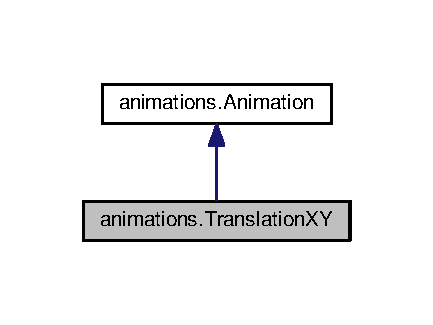
\includegraphics[width=208pt]{classanimations_1_1TranslationXY__inherit__graph}
\end{center}
\end{figure}


Collaboration diagram for animations.\+Translation\+XY\+:\nopagebreak
\begin{figure}[H]
\begin{center}
\leavevmode
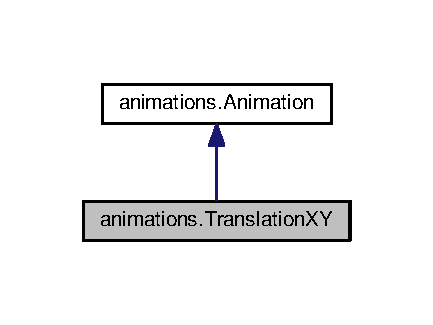
\includegraphics[width=208pt]{classanimations_1_1TranslationXY__coll__graph}
\end{center}
\end{figure}
\subsection*{Public Member Functions}
\begin{DoxyCompactItemize}
\item 
def {\bfseries \+\_\+\+\_\+init\+\_\+\+\_\+} (self, bdr\+\_\+handler, blender\+\_\+object, frames)\hypertarget{classanimations_1_1TranslationXY_afe2004ca86af674725eb1ee05f0d9212}{}\label{classanimations_1_1TranslationXY_afe2004ca86af674725eb1ee05f0d9212}

\end{DoxyCompactItemize}
\subsection*{Static Public Member Functions}
\begin{DoxyCompactItemize}
\item 
def {\bfseries get\+\_\+start\+\_\+rotation} ()\hypertarget{classanimations_1_1TranslationXY_a2fa5e14138697e9234b877e9e73a09d4}{}\label{classanimations_1_1TranslationXY_a2fa5e14138697e9234b877e9e73a09d4}

\item 
def {\bfseries get\+\_\+start\+\_\+position} ()\hypertarget{classanimations_1_1TranslationXY_ac94d11d8de6e13b8c27d4a66f8454ecc}{}\label{classanimations_1_1TranslationXY_ac94d11d8de6e13b8c27d4a66f8454ecc}

\end{DoxyCompactItemize}
\subsection*{Static Public Attributes}
\begin{DoxyCompactItemize}
\item 
string {\bfseries interpolation} = \textquotesingle{}L\+I\+N\+E\+AR\textquotesingle{}\hypertarget{classanimations_1_1TranslationXY_a8af4befa781354425d0cc12a4dea8377}{}\label{classanimations_1_1TranslationXY_a8af4befa781354425d0cc12a4dea8377}

\end{DoxyCompactItemize}


The documentation for this class was generated from the following file\+:\begin{DoxyCompactItemize}
\item 
/home/sebastian/catkin\+\_\+ws/src/animation\+\_\+render/scripts/framework/animations.\+py\end{DoxyCompactItemize}

\hypertarget{classanimations_1_1TranslationXYrotated}{}\section{animations.\+Translation\+X\+Yrotated Class Reference}
\label{classanimations_1_1TranslationXYrotated}\index{animations.\+Translation\+X\+Yrotated@{animations.\+Translation\+X\+Yrotated}}


Inheritance diagram for animations.\+Translation\+X\+Yrotated\+:\nopagebreak
\begin{figure}[H]
\begin{center}
\leavevmode
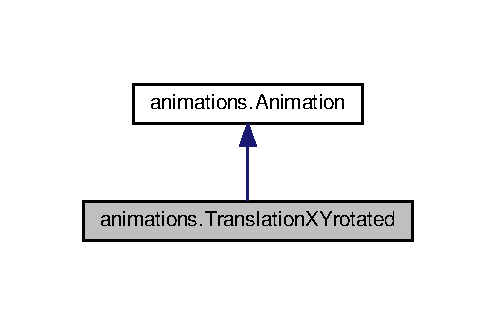
\includegraphics[width=238pt]{classanimations_1_1TranslationXYrotated__inherit__graph}
\end{center}
\end{figure}


Collaboration diagram for animations.\+Translation\+X\+Yrotated\+:\nopagebreak
\begin{figure}[H]
\begin{center}
\leavevmode
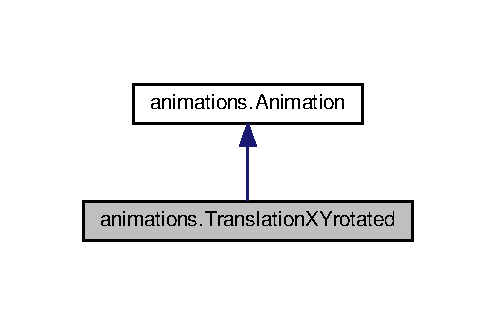
\includegraphics[width=238pt]{classanimations_1_1TranslationXYrotated__coll__graph}
\end{center}
\end{figure}
\subsection*{Public Member Functions}
\begin{DoxyCompactItemize}
\item 
def {\bfseries \+\_\+\+\_\+init\+\_\+\+\_\+} (self, bdr\+\_\+handler, blender\+\_\+object, frames)\hypertarget{classanimations_1_1TranslationXYrotated_ac8f4d6d489fc2a0d1d61c83efef61860}{}\label{classanimations_1_1TranslationXYrotated_ac8f4d6d489fc2a0d1d61c83efef61860}

\end{DoxyCompactItemize}
\subsection*{Static Public Member Functions}
\begin{DoxyCompactItemize}
\item 
def {\bfseries get\+\_\+start\+\_\+position} ()\hypertarget{classanimations_1_1TranslationXYrotated_a96ab51c4c29c1f60ab6c9b79f991cbd0}{}\label{classanimations_1_1TranslationXYrotated_a96ab51c4c29c1f60ab6c9b79f991cbd0}

\item 
def {\bfseries get\+\_\+start\+\_\+rotation} ()\hypertarget{classanimations_1_1TranslationXYrotated_aee8c304b43574876eea002b7a9b7ad0d}{}\label{classanimations_1_1TranslationXYrotated_aee8c304b43574876eea002b7a9b7ad0d}

\end{DoxyCompactItemize}
\subsection*{Static Public Attributes}
\begin{DoxyCompactItemize}
\item 
string {\bfseries interpolation} = \textquotesingle{}Q\+U\+AD\textquotesingle{}\hypertarget{classanimations_1_1TranslationXYrotated_a06501d8a2da0f01d5750642d41ec5f76}{}\label{classanimations_1_1TranslationXYrotated_a06501d8a2da0f01d5750642d41ec5f76}

\end{DoxyCompactItemize}


The documentation for this class was generated from the following file\+:\begin{DoxyCompactItemize}
\item 
/home/sebastian/catkin\+\_\+ws/src/animation\+\_\+render/scripts/framework/animations.\+py\end{DoxyCompactItemize}

\hypertarget{classanimations_1_1TranslationY}{}\section{animations.\+TranslationY Class Reference}
\label{classanimations_1_1TranslationY}\index{animations.\+TranslationY@{animations.\+TranslationY}}


Inheritance diagram for animations.\+TranslationY\+:\nopagebreak
\begin{figure}[H]
\begin{center}
\leavevmode
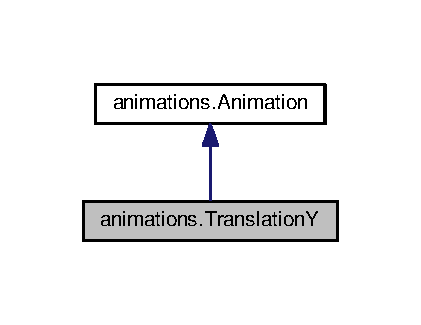
\includegraphics[width=202pt]{classanimations_1_1TranslationY__inherit__graph}
\end{center}
\end{figure}


Collaboration diagram for animations.\+TranslationY\+:\nopagebreak
\begin{figure}[H]
\begin{center}
\leavevmode
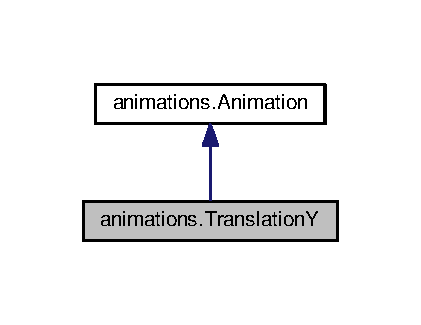
\includegraphics[width=202pt]{classanimations_1_1TranslationY__coll__graph}
\end{center}
\end{figure}
\subsection*{Public Member Functions}
\begin{DoxyCompactItemize}
\item 
def {\bfseries \+\_\+\+\_\+init\+\_\+\+\_\+} (self, bdr\+\_\+handler, blender\+\_\+object, frames)\hypertarget{classanimations_1_1TranslationY_ae8fa8e1b9e86470fb55294820b515cfa}{}\label{classanimations_1_1TranslationY_ae8fa8e1b9e86470fb55294820b515cfa}

\end{DoxyCompactItemize}
\subsection*{Static Public Member Functions}
\begin{DoxyCompactItemize}
\item 
def {\bfseries get\+\_\+start\+\_\+rotation} ()\hypertarget{classanimations_1_1TranslationY_a2e584d49e504ad24c5b828da26542ea3}{}\label{classanimations_1_1TranslationY_a2e584d49e504ad24c5b828da26542ea3}

\item 
def {\bfseries get\+\_\+start\+\_\+position} ()\hypertarget{classanimations_1_1TranslationY_adb1b8ddce977d79c6185cba374c30c12}{}\label{classanimations_1_1TranslationY_adb1b8ddce977d79c6185cba374c30c12}

\end{DoxyCompactItemize}
\subsection*{Static Public Attributes}
\begin{DoxyCompactItemize}
\item 
string {\bfseries interpolation} = \textquotesingle{}Q\+U\+AD\textquotesingle{}\hypertarget{classanimations_1_1TranslationY_a089db7389078d26a0933ca41af9dd12f}{}\label{classanimations_1_1TranslationY_a089db7389078d26a0933ca41af9dd12f}

\end{DoxyCompactItemize}


The documentation for this class was generated from the following file\+:\begin{DoxyCompactItemize}
\item 
/home/sebastian/catkin\+\_\+ws/src/animation\+\_\+render/scripts/framework/animations.\+py\end{DoxyCompactItemize}

\hypertarget{classanimations_1_1TranslationZ}{}\section{animations.\+TranslationZ Class Reference}
\label{classanimations_1_1TranslationZ}\index{animations.\+TranslationZ@{animations.\+TranslationZ}}


Inheritance diagram for animations.\+TranslationZ\+:\nopagebreak
\begin{figure}[H]
\begin{center}
\leavevmode
\includegraphics[width=201pt]{classanimations_1_1TranslationZ__inherit__graph}
\end{center}
\end{figure}


Collaboration diagram for animations.\+TranslationZ\+:\nopagebreak
\begin{figure}[H]
\begin{center}
\leavevmode
\includegraphics[width=201pt]{classanimations_1_1TranslationZ__coll__graph}
\end{center}
\end{figure}
\subsection*{Public Member Functions}
\begin{DoxyCompactItemize}
\item 
def {\bfseries \+\_\+\+\_\+init\+\_\+\+\_\+} (self, bdr\+\_\+handler, blender\+\_\+object, frames)\hypertarget{classanimations_1_1TranslationZ_ae0da43143baf3a4b80e88d476083446b}{}\label{classanimations_1_1TranslationZ_ae0da43143baf3a4b80e88d476083446b}

\end{DoxyCompactItemize}
\subsection*{Static Public Member Functions}
\begin{DoxyCompactItemize}
\item 
def {\bfseries get\+\_\+start\+\_\+position} ()\hypertarget{classanimations_1_1TranslationZ_ae09c0738b5727161a75b22cb7638656a}{}\label{classanimations_1_1TranslationZ_ae09c0738b5727161a75b22cb7638656a}

\item 
def {\bfseries get\+\_\+start\+\_\+rotation} ()\hypertarget{classanimations_1_1TranslationZ_a3324d14e040bc7674eb947f8563e56ac}{}\label{classanimations_1_1TranslationZ_a3324d14e040bc7674eb947f8563e56ac}

\end{DoxyCompactItemize}
\subsection*{Static Public Attributes}
\begin{DoxyCompactItemize}
\item 
string {\bfseries interpolation} = \textquotesingle{}L\+I\+N\+E\+AR\textquotesingle{}\hypertarget{classanimations_1_1TranslationZ_a02eae8d9682acc8bd0f915c6322b6456}{}\label{classanimations_1_1TranslationZ_a02eae8d9682acc8bd0f915c6322b6456}

\end{DoxyCompactItemize}


The documentation for this class was generated from the following file\+:\begin{DoxyCompactItemize}
\item 
/home/sebastian/catkin\+\_\+ws/src/animation\+\_\+render/scripts/framework/animations.\+py\end{DoxyCompactItemize}

\hypertarget{structVideoOptions}{}\section{Video\+Options Struct Reference}
\label{structVideoOptions}\index{Video\+Options@{Video\+Options}}
\subsection*{Public Attributes}
\begin{DoxyCompactItemize}
\item 
int {\bfseries width}\hypertarget{structVideoOptions_ad47a8f090805a349fc6f200d21c71549}{}\label{structVideoOptions_ad47a8f090805a349fc6f200d21c71549}

\item 
int {\bfseries height}\hypertarget{structVideoOptions_a9031cd944b0dd5c6e6c135afb0db5b26}{}\label{structVideoOptions_a9031cd944b0dd5c6e6c135afb0db5b26}

\item 
int {\bfseries fps}\hypertarget{structVideoOptions_a73674e8c88aa4f459c127511be49c0b2}{}\label{structVideoOptions_a73674e8c88aa4f459c127511be49c0b2}

\item 
int {\bfseries frames}\hypertarget{structVideoOptions_a644e265827a217ce4e7eabc2f226904d}{}\label{structVideoOptions_a644e265827a217ce4e7eabc2f226904d}

\item 
double {\bfseries sensor\+\_\+width}\hypertarget{structVideoOptions_ae16bb057999c1278e501d27f35cc0b85}{}\label{structVideoOptions_ae16bb057999c1278e501d27f35cc0b85}

\item 
double {\bfseries focal\+\_\+length}\hypertarget{structVideoOptions_a13b51ddc57b1ab2a3696d9edbcb74107}{}\label{structVideoOptions_a13b51ddc57b1ab2a3696d9edbcb74107}

\end{DoxyCompactItemize}


The documentation for this struct was generated from the following file\+:\begin{DoxyCompactItemize}
\item 
/home/sebastian/catkin\+\_\+ws/src/animation\+\_\+render/src/pythoncaller.\+h\end{DoxyCompactItemize}

\hypertarget{classVideoStream}{}\section{Video\+Stream Class Reference}
\label{classVideoStream}\index{Video\+Stream@{Video\+Stream}}
\subsection*{Public Member Functions}
\begin{DoxyCompactItemize}
\item 
{\bfseries Video\+Stream} (ros\+::\+Node\+Handle rosH)\hypertarget{classVideoStream_ab3287a533657a03cfb293793962faf3c}{}\label{classVideoStream_ab3287a533657a03cfb293793962faf3c}

\item 
bool \hyperlink{classVideoStream_ab8d19b1d9d1156fb9d12ada5ce6409bb}{open\+Stream} (std\+::string path, \hyperlink{structVideoOptions}{Video\+Options} options)
\begin{DoxyCompactList}\small\item\em open\+Stream Reads video file and streams it over camera topic \end{DoxyCompactList}\end{DoxyCompactItemize}


\subsection{Member Function Documentation}
\index{Video\+Stream@{Video\+Stream}!open\+Stream@{open\+Stream}}
\index{open\+Stream@{open\+Stream}!Video\+Stream@{Video\+Stream}}
\subsubsection[{\texorpdfstring{open\+Stream(std\+::string path, Video\+Options options)}{openStream(std::string path, VideoOptions options)}}]{\setlength{\rightskip}{0pt plus 5cm}bool Video\+Stream\+::open\+Stream (
\begin{DoxyParamCaption}
\item[{std\+::string}]{path, }
\item[{{\bf Video\+Options}}]{options}
\end{DoxyParamCaption}
)}\hypertarget{classVideoStream_ab8d19b1d9d1156fb9d12ada5ce6409bb}{}\label{classVideoStream_ab8d19b1d9d1156fb9d12ada5ce6409bb}


open\+Stream Reads video file and streams it over camera topic 


\begin{DoxyParams}{Parameters}
{\em path} & Path of video file \\
\hline
\end{DoxyParams}


The documentation for this class was generated from the following files\+:\begin{DoxyCompactItemize}
\item 
/home/sebastian/catkin\+\_\+ws/src/animation\+\_\+render/src/videostream.\+h\item 
/home/sebastian/catkin\+\_\+ws/src/animation\+\_\+render/src/videostream.\+cpp\end{DoxyCompactItemize}

%--- End generated contents ---

% Index
\backmatter
\newpage
\phantomsection
\clearemptydoublepage
\addcontentsline{toc}{chapter}{Index}
\printindex

\end{document}
